\documentclass[compress, serif]{beamer}
%\documentclass [serif]{beamer} % ``serif'' option for CM

\useoutertheme[subsection=false]{miniframes}
\usepackage{etoolbox}
\makeatletter
\patchcmd{\slideentry}{\advance\beamer@xpos by1\relax}{}{}{}
\def\beamer@subsectionentry#1#2#3#4#5{\advance\beamer@xpos by1\relax}%
\makeatother

%\documentclass{beamer}
\usetheme{Singapore}
\usecolortheme{seagull}
\usepackage{pgfplots}
\usetikzlibrary{arrows,shapes,positioning}
\graphicspath{{graphics/}}
\usepackage{xcolor}
%\setbeamertemplate{navigation symbols}{\thepage}
\usepackage{tikz}
\usepackage{transparent}
\usepackage{xspace}
\usepackage{verbatim}

\makeatletter
\@addtoreset{subfigure}{framenumber}% subfigure counter resets every frame
\makeatother
\usetikzlibrary{arrows,shapes}
\tikzstyle{every picture}+=[remember picture]
\tikzstyle{na} = [baseline=-.5ex]
\setbeamercovered{dynamic}
\usepackage{tabularx}
\usepackage[scriptsize]{subfigure}
\usepackage[absolute,overlay]{textpos}
\newcommand{\lenitem}[2][.7\linewidth]{\parbox[t]{#1}{\strut #2\strut}}
\definecolor{niceRed}{rgb}{228,59,59}
\newcommand{\GeV}{\ensuremath{\,\text{Ge\hspace{-.08em}V}}\xspace}
\newcommand{\gev}{\GeV}
\newcommand{\TeV}{\ensuremath{\,\text{Te\hspace{-.08em}V}}\xspace}
\newcommand{\njet}{\ensuremath{n_{\text{jet}}}\xspace}
\newcommand{\njetlow}{\ensuremath{2 \leq \njet \leq 3}\xspace}
\newcommand{\njethigh}{\ensuremath{\njet \geq 4}\xspace}
\newcommand{\npre}{\ensuremath{N_{\textrm{pred}}}\xspace}
\newcommand{\nobs}{\ensuremath{N_{\textrm{obs}}}\xspace}
\newcommand{\gj}{\ensuremath{\gamma} + jets\xspace}
\newcommand{\mj}{\ensuremath{\mu} + jets\xspace}
\newcommand{\nb}{\ensuremath{n_{\text{b}}}\xspace}
\newcommand {\ie}{\mbox{i.e.}\xspace}     %i.e.
\newcommand{\ra}{\ensuremath{\rightarrow}}
\newcommand{\fZinv}[1]{\ensuremath{f_{\rm Zinv}^{#1}}\xspace}
\newcommand{\zInv}[1]{\ensuremath{Z_{\rm inv}^{#1}}\xspace}
\newcommand{\tev}{\ensuremath{\,\text{Te\hspace{-.08em}V}}\xspace}
\newcommand{\st}{\ensuremath{\tilde{\rm t}}\xspace}
\newcommand{\VEtmiss}{\ensuremath{{\vec E}_{\mathrm{T}}^{\text{miss}}}\xspace}
\newcommand{\znunu}{\ensuremath{{\text Z} \ra \nu\bar{\nu}}\xspace}
\newcommand{\ttj}{\ensuremath{\rm{t}\bar{\rm{t}} + jets}\xspace}
\newcommand{\wj}{\ensuremath{\rm W + jets}\xspace}
\newcommand{\wlnu}{\ensuremath{{\text W}\!\ra\!l\nu}\xspace}
\newcommand{\zj}{\ensuremath{\rm Z + jets}\xspace}
\providecommand{\e}[1]{\ensuremath{\times 10^{#1}}}
\newcommand{\dyll}{\ensuremath{{\text Z/\gamma^{*}} \rightarrow l^{+}l^{-}}\xspace}
\addtobeamertemplate{navigation symbols}{}{%
    \usebeamerfont{footline}%
    \usebeamercolor[fg]{footline}%
    \hspace{1em}%
    \insertframenumber/\inserttotalframenumber
}


%\def\vecmet{\mbox{$\vec{\not\!\!E_\text{T}}$}} %missing ET vector
\def\scalht{\mbox{$H_\text{T}$}\xspace}
\def\met{\mbox{$\not\!\!E_\text{T}$}\xspace}
\newcommand{\alphat}{\ensuremath{\alpha_{\text{T}}}\xspace}
\newcommand{\Et}{\ensuremath{{E_{\text T}}}\xspace}
\def\mht{\mbox{$\not\!\!H_\text{T}$}\xspace}
\newcommand{\pt}{\ensuremath{p_{\mathrm{T}}}\xspace}

\begin{document}

\title{Search for New Physics in All-hadronic Events with AlphaT in 8 TeV Data with CMS}
\author{Y.~Eshaq\\}
%\today}
\date{December 5, 2014}
%\date{\today}
%\setbeamertemplate{footline}{}

\frame{\titlepage}

%%%%%%%%%%%%%%%%%%%%%%%%%%%%
%%%%%%%% OUTLINE %%%%%%%%%%%
%%%%%%%%%%%%%%%%%%%%%%%%%%%%
\frame{
  \frametitle{Outline}

\begin{itemize}
\item The Standard Model (SM), Supersymmetry (SUSY) \tikz[na] \node[coordinate] (s1) {}; 
\end{itemize}
~\\

\begin{center}
Search for 
\tikz[baseline]{ \node[fill=red!20,anchor=base,rounded corners=2pt]
  (d1) { New Physics}; }
in All-hadronic Events with AlphaT in 8~TeV Data with CMS
\end{center}

\begin{tikzpicture}[overlay]
\path[->] (s1) edge [out=-90,in=45] (d1); 
\end{tikzpicture}
}

\frame{
  \frametitle{Outline}

\begin{itemize}
\item The Standard Model (SM), Supersymmetry (SUSY) \tikz[na] \node[coordinate] (s1) {}; 
\item Large Hadron Collider, Compact Muon Solenoid (CMS) \tikz[na] \node[coordinate] (s3) {};
\end{itemize}
~\\

\begin{center}
Search for New Physics in All-hadronic Events with AlphaT in 
\tikz[baseline]{ \node[fill=blue!20,anchor=base,rounded corners=2pt]
  (d4) {8~TeV Data}; } with
\tikz[baseline]{ \node[fill=blue!20,anchor=base,rounded corners=2pt]
  (d5) {CMS}; }
\end{center}

\begin{tikzpicture}[overlay]
\path[->] (s3) edge [out=-115, in=45] (d4);
\path[->] (s3) edge [out=-15, in=0] (d5);
\end{tikzpicture}
}

\frame{
  \frametitle{Outline}

\begin{itemize}
\item The Standard Model (SM), Supersymmetry (SUSY) \tikz[na] \node[coordinate] (s1) {}; 
\item Large Hadron Collider, Compact Muon Solenoid (CMS) \tikz[na] \node[coordinate] (s3) {};
\item Search strategy, analysis ingredients \tikz[na] \node[coordinate] (s2) {};
\end{itemize}
~\\

\begin{center}
\tikz[baseline]{ \node[fill=green!40,anchor=base,rounded corners=2pt]
  (d2) {Search}; } for New Physics in
%\tikz[baseline]{ \node[fill=red!20,anchor=base,rounded corners=2pt]
%  (d1) { New Physics}; } in 
\tikz[baseline]{ \node[fill=green!40,anchor=base,rounded corners=2pt]
  (d3) {All-hadronic}; } Events with 
\tikz[baseline]{ \node[fill=green!40,anchor=base,rounded corners=2pt]
  (d4) {AlphaT}; } in 8~TeV Data with CMS
%\tikz[baseline]{ \node[fill=green!20,anchor=base,rounded corners=2pt]
%  (d5) {CMS}; } 
\end{center}

\begin{tikzpicture}[overlay]
\path[->] (s2) edge [out=-135, in=45] (d2);
\path[->] (s2) edge [out=-90, in=105] (d3);
\path[->] (s2) edge [out=-25, in=115] (d4);
\end{tikzpicture}
}

\frame{
  \frametitle{Outline}

\begin{itemize}
\item The Standard Model (SM), Supersymmetry (SUSY) \tikz[na] \node[coordinate] (s1) {}; 
\item Large Hadron Collider (LHC), Compact Muon Solenoid (CMS) \tikz[na] \node[coordinate] (s3) {};
\item Search strategy, analysis ingredients \tikz[na] \node[coordinate] (s2) {};
\end{itemize}
~\\

\begin{center}
\tikz[baseline]{ \node[fill=blue!20,anchor=base,rounded corners=2pt]
  (d2) {Search for New Physics in All-hadronic Events with AlphaT};}
\tikz[baseline]{ \node[fill=blue!20,anchor=base,rounded corners=2pt]{in 8~TeV Data with CMS}; }
\end{center}

\begin{itemize}
\item Results \tikz[na] \node[coordinate] (s6) {}; 
\end{itemize}

}
%%%%%%%%%%%%%%%%%%%%%%%%%%%%
%%%%%%%% OUTLINE %%%%%%%%%%%
%%%%%%%%%%%%%%%%%%%%%%%%%%%%
\section{Motivation}
\subsection{Standard Model}
\frame{
  \frametitle{The Standard Model}
\begin{columns}[lc]
\column{0.5\paperwidth}
\begin{itemize}
  \item Very succesful model:
    \begin{itemize}
    \item Predicts all known particles and interaction
    \item Muon Anomalous Magnetic Moment
      \item Z Boson $\rightarrow$ cross section, branching fraction
    \end{itemize}
  \item The Standard Model doesn't explain everything
\end{itemize}
\column{0.5\paperwidth}
%\begin{textblock*}{5cm}(6cm,2cm) % {block width} (coords)
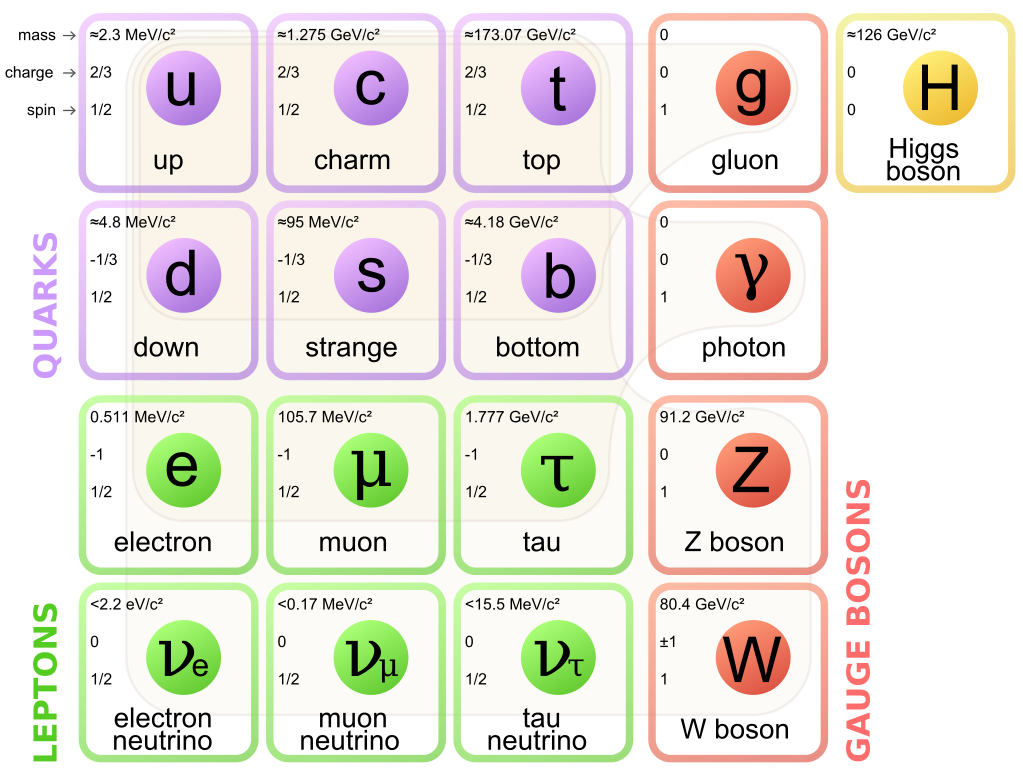
\includegraphics[width=1.0\textwidth,]{../figures/Standard_Model_of_Elementary_Particles.png}
%\end{textblock*}
\end{columns}
}

\frame{
\frametitle{Shortcomings of the SM}
\begin{itemize}
\setlength{\itemsep}{8pt}
\item Dark Matter: 96\% of matter remains unexplained 
\item Gravity: The SM becomes invalid above $M_{plank} > 10^{19}~GeV$ where gravity can't be ignored
\item Massless Neurinos
\item Does not allow for unification of forces
\item Divergent corrections to the Higgs mass - ``Hiearchy problem''
\end{itemize}
\begin{equation*}
\underbrace{\mathrm{m}^2_{\text{physical}}}_{\text{what we measure}} = \underbrace{\mathrm{m}_{\mathrm{h}}^2}_{\text{tree level}} \;+\; \underbrace{\frac{3\lambda}{8\pi}\Lambda^2}_{\text{1-loop}} \;-\; \underbrace{\frac{3\lambda}{8\pi}\mathrm{m}_{\mathrm{h}}^2\text{log}\left(\frac{\Lambda^2+\mathrm{m}_{\mathrm{h}}^2}{\mathrm{m}_{\mathrm{h}}^2}\right)}_{\text{much smaller than} \Lambda^2}
\end{equation*}

%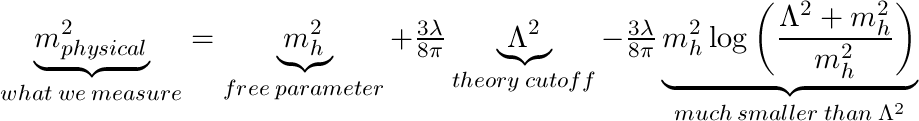
\includegraphics[width=.85\paperwidth,]{../figures/higgs_MassCorrection.png}

%\begin{itemize}
%\item effective theory \pause
%\end{itemize}
\color{red!80}{Any extension of th SM should attempt to solve these shortcomings...}
}
\subsection{SUSY}
\frame{
\frametitle{Supersymmetry}
\begin{center}
\color{red!80}{A proposed symmetry of spin}
\end{center}
\begin{center}
\begin{textblock*}{3cm}(-0.5cm,4.5cm) % {block width} (coords)
\color{blue!80}{spin 1/2}
\end{textblock*}
\begin{textblock*}{3cm}(10cm,4.5cm) % {block width} (coords)
\color{blue!80}{spin 0}
\end{textblock*}
\begin{textblock*}{3cm}(0.5cm,7cm) % {block width} (coords)
\color{blue!80}{spin 1}
\end{textblock*}
\begin{textblock*}{3cm}(10.1cm,7cm) % {block width} (coords)
\color{blue!80}{spin 1/2}
\end{textblock*}
\color{black}
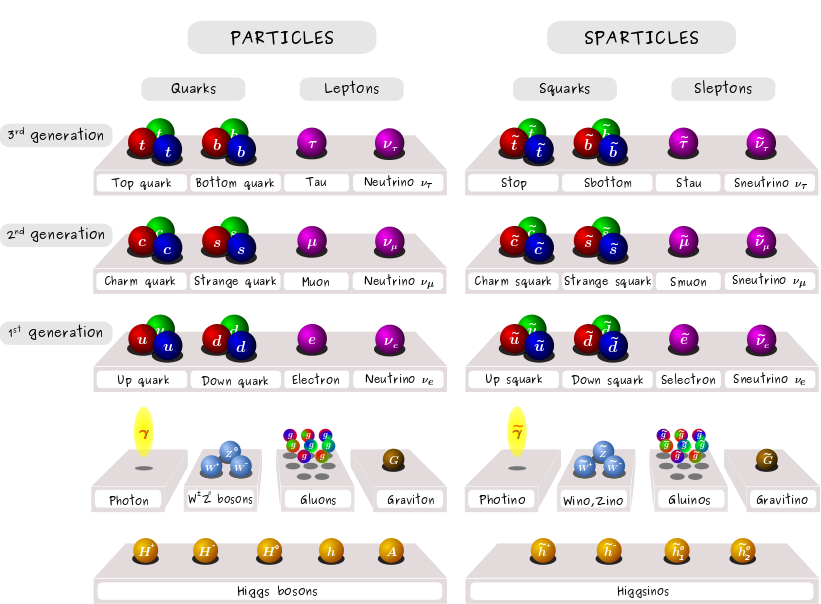
\includegraphics[width=.6\paperwidth,]{../figures/susy_spectrum.png}\\

\small{Higgsino $\Longleftrightarrow$ Bino/Wino = 4 Neutralino ($\tilde{\chi}_{1-4}^0$)\\
Higgsino $\Longleftrightarrow$ Wino = 2 Charginos ($\tilde{\chi}_{1-2}^+$)}
\end{center}
}
\color{black}
\frame{
\frametitle{Supersymmetry}
Supersymmetry is theoretically well motivated:
~\\
\begin{itemize}
\setlength{\itemsep}{10pt}
\item It provides a solution to the \\hierarchy problem 
\item Unifies the gauge couplings 
\begin{textblock*}{5cm}(6.8cm,3.2cm) % {block width} (coords)
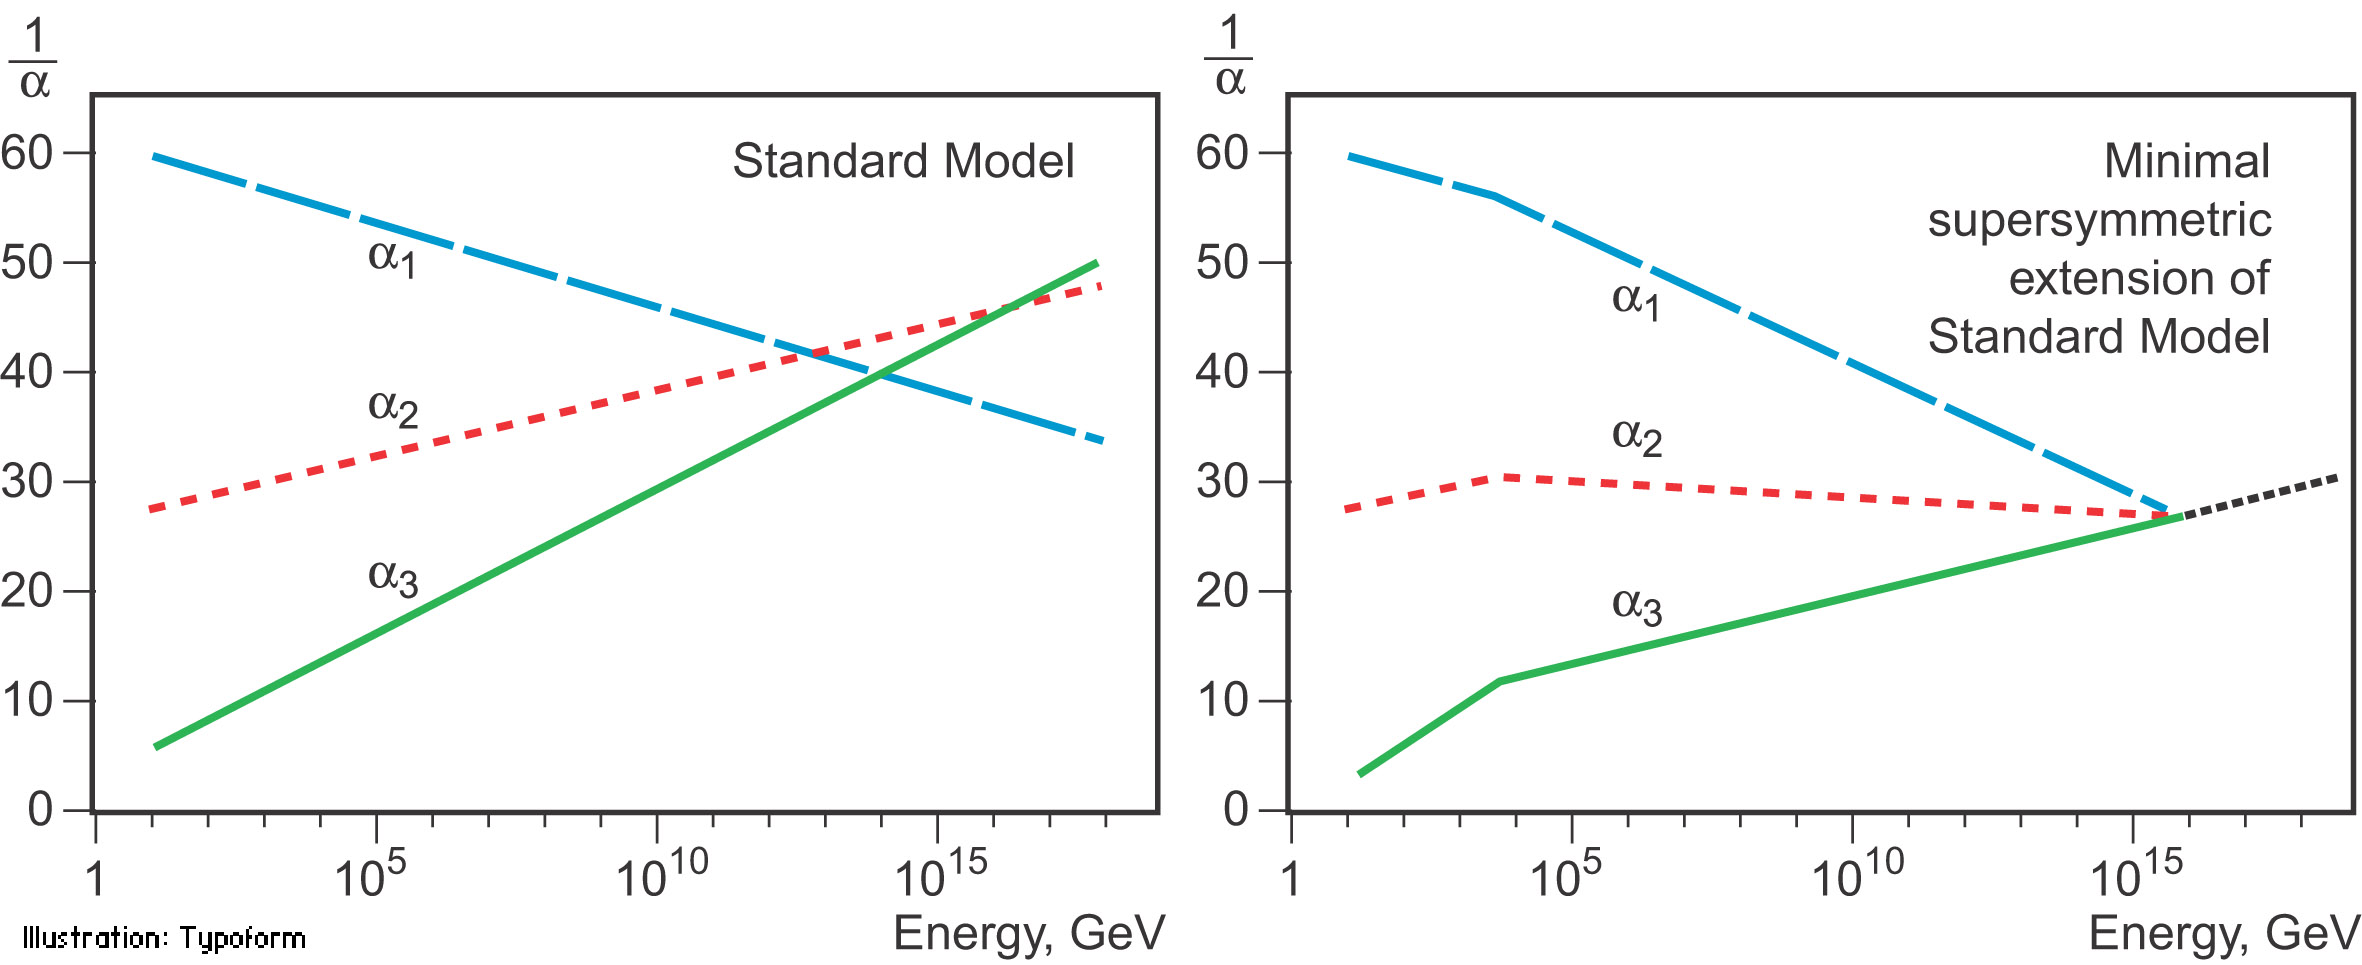
\includegraphics[width=.45\paperwidth,]{../figures/phypub4highen.jpg}
\end{textblock*}
\item Provides a candidate for \\Dark Matter
\item Provides additional loop \\corrections ot the Higgs mass which cancel the qudratic divergence! 
\end{itemize}
\begin{center}
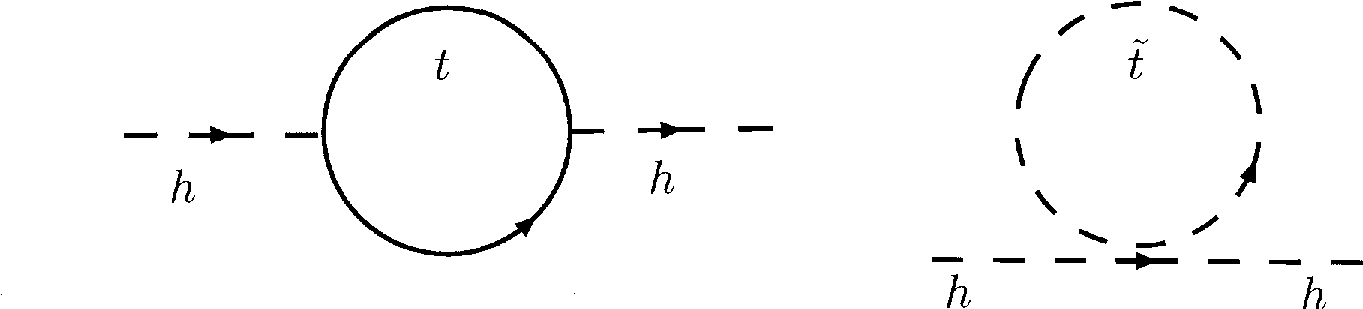
\includegraphics[width=.45\paperwidth,]{../figures/top_stop_higgsloop.png}
\end{center}
}
\section{The Expirement}
\subsection{LHC}
\frame{
\frametitle{The Large Hadron Collider}
\begin{itemize}
\setlength{\itemsep}{15pt}
\item proton-proton (pp) collider \\housed 
100m underground in a \\27km circular tunnel

\item 2808 ``bunches'' of protons \\measuring 
$16~\mu$m transversely \\and $\sim30$~cm long
orbit 7~m \\apart

\item $10^{11}$ protons per bunch lead to \\around 20 collsions per \\beam crossing.
\end{itemize}

\begin{textblock*}{5cm}(7.3cm,1.6cm) % {block width} (coords)
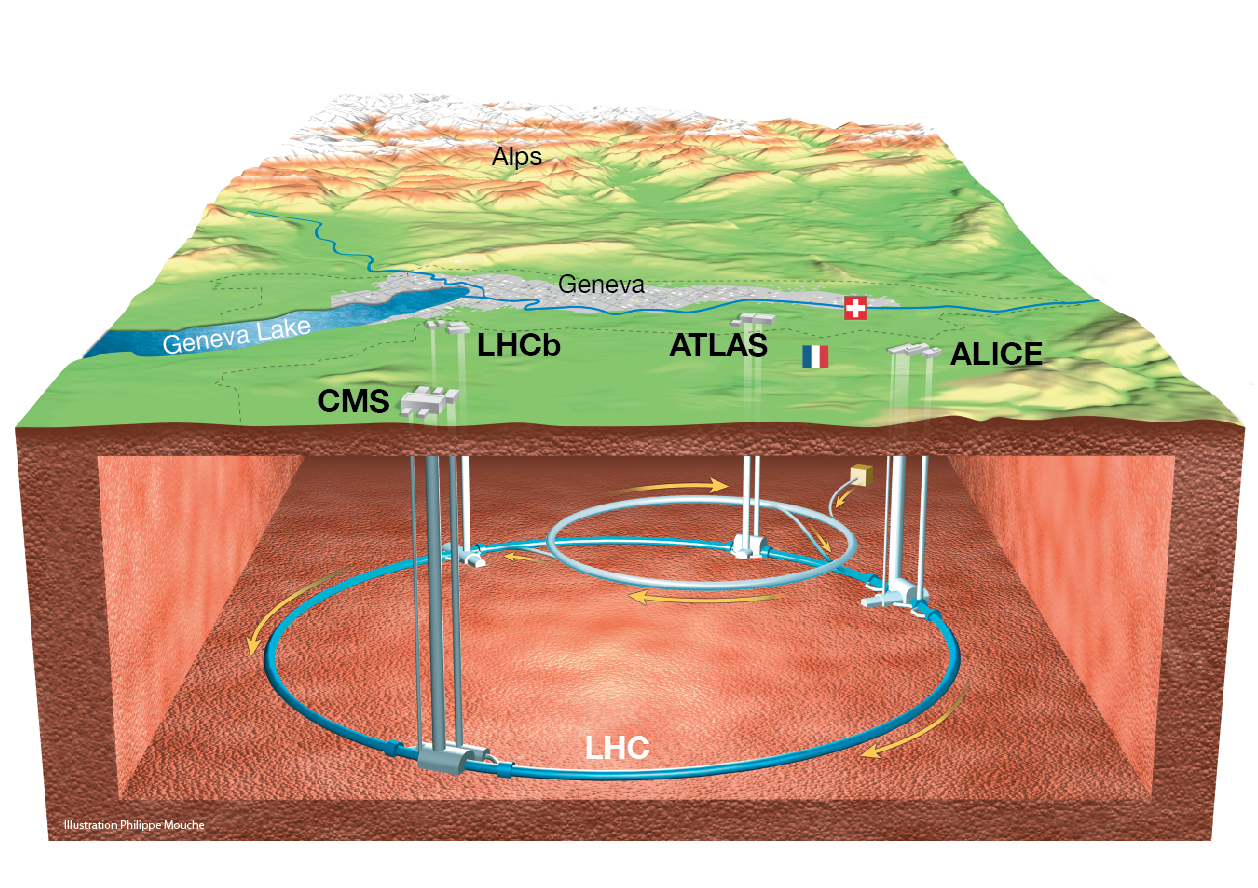
\includegraphics[width=.4\paperwidth,]{../figures/CERN_hiRes.png}
\end{textblock*}
\begin{textblock*}{5cm}(7.1cm,5.2cm) % {block width} (coords)
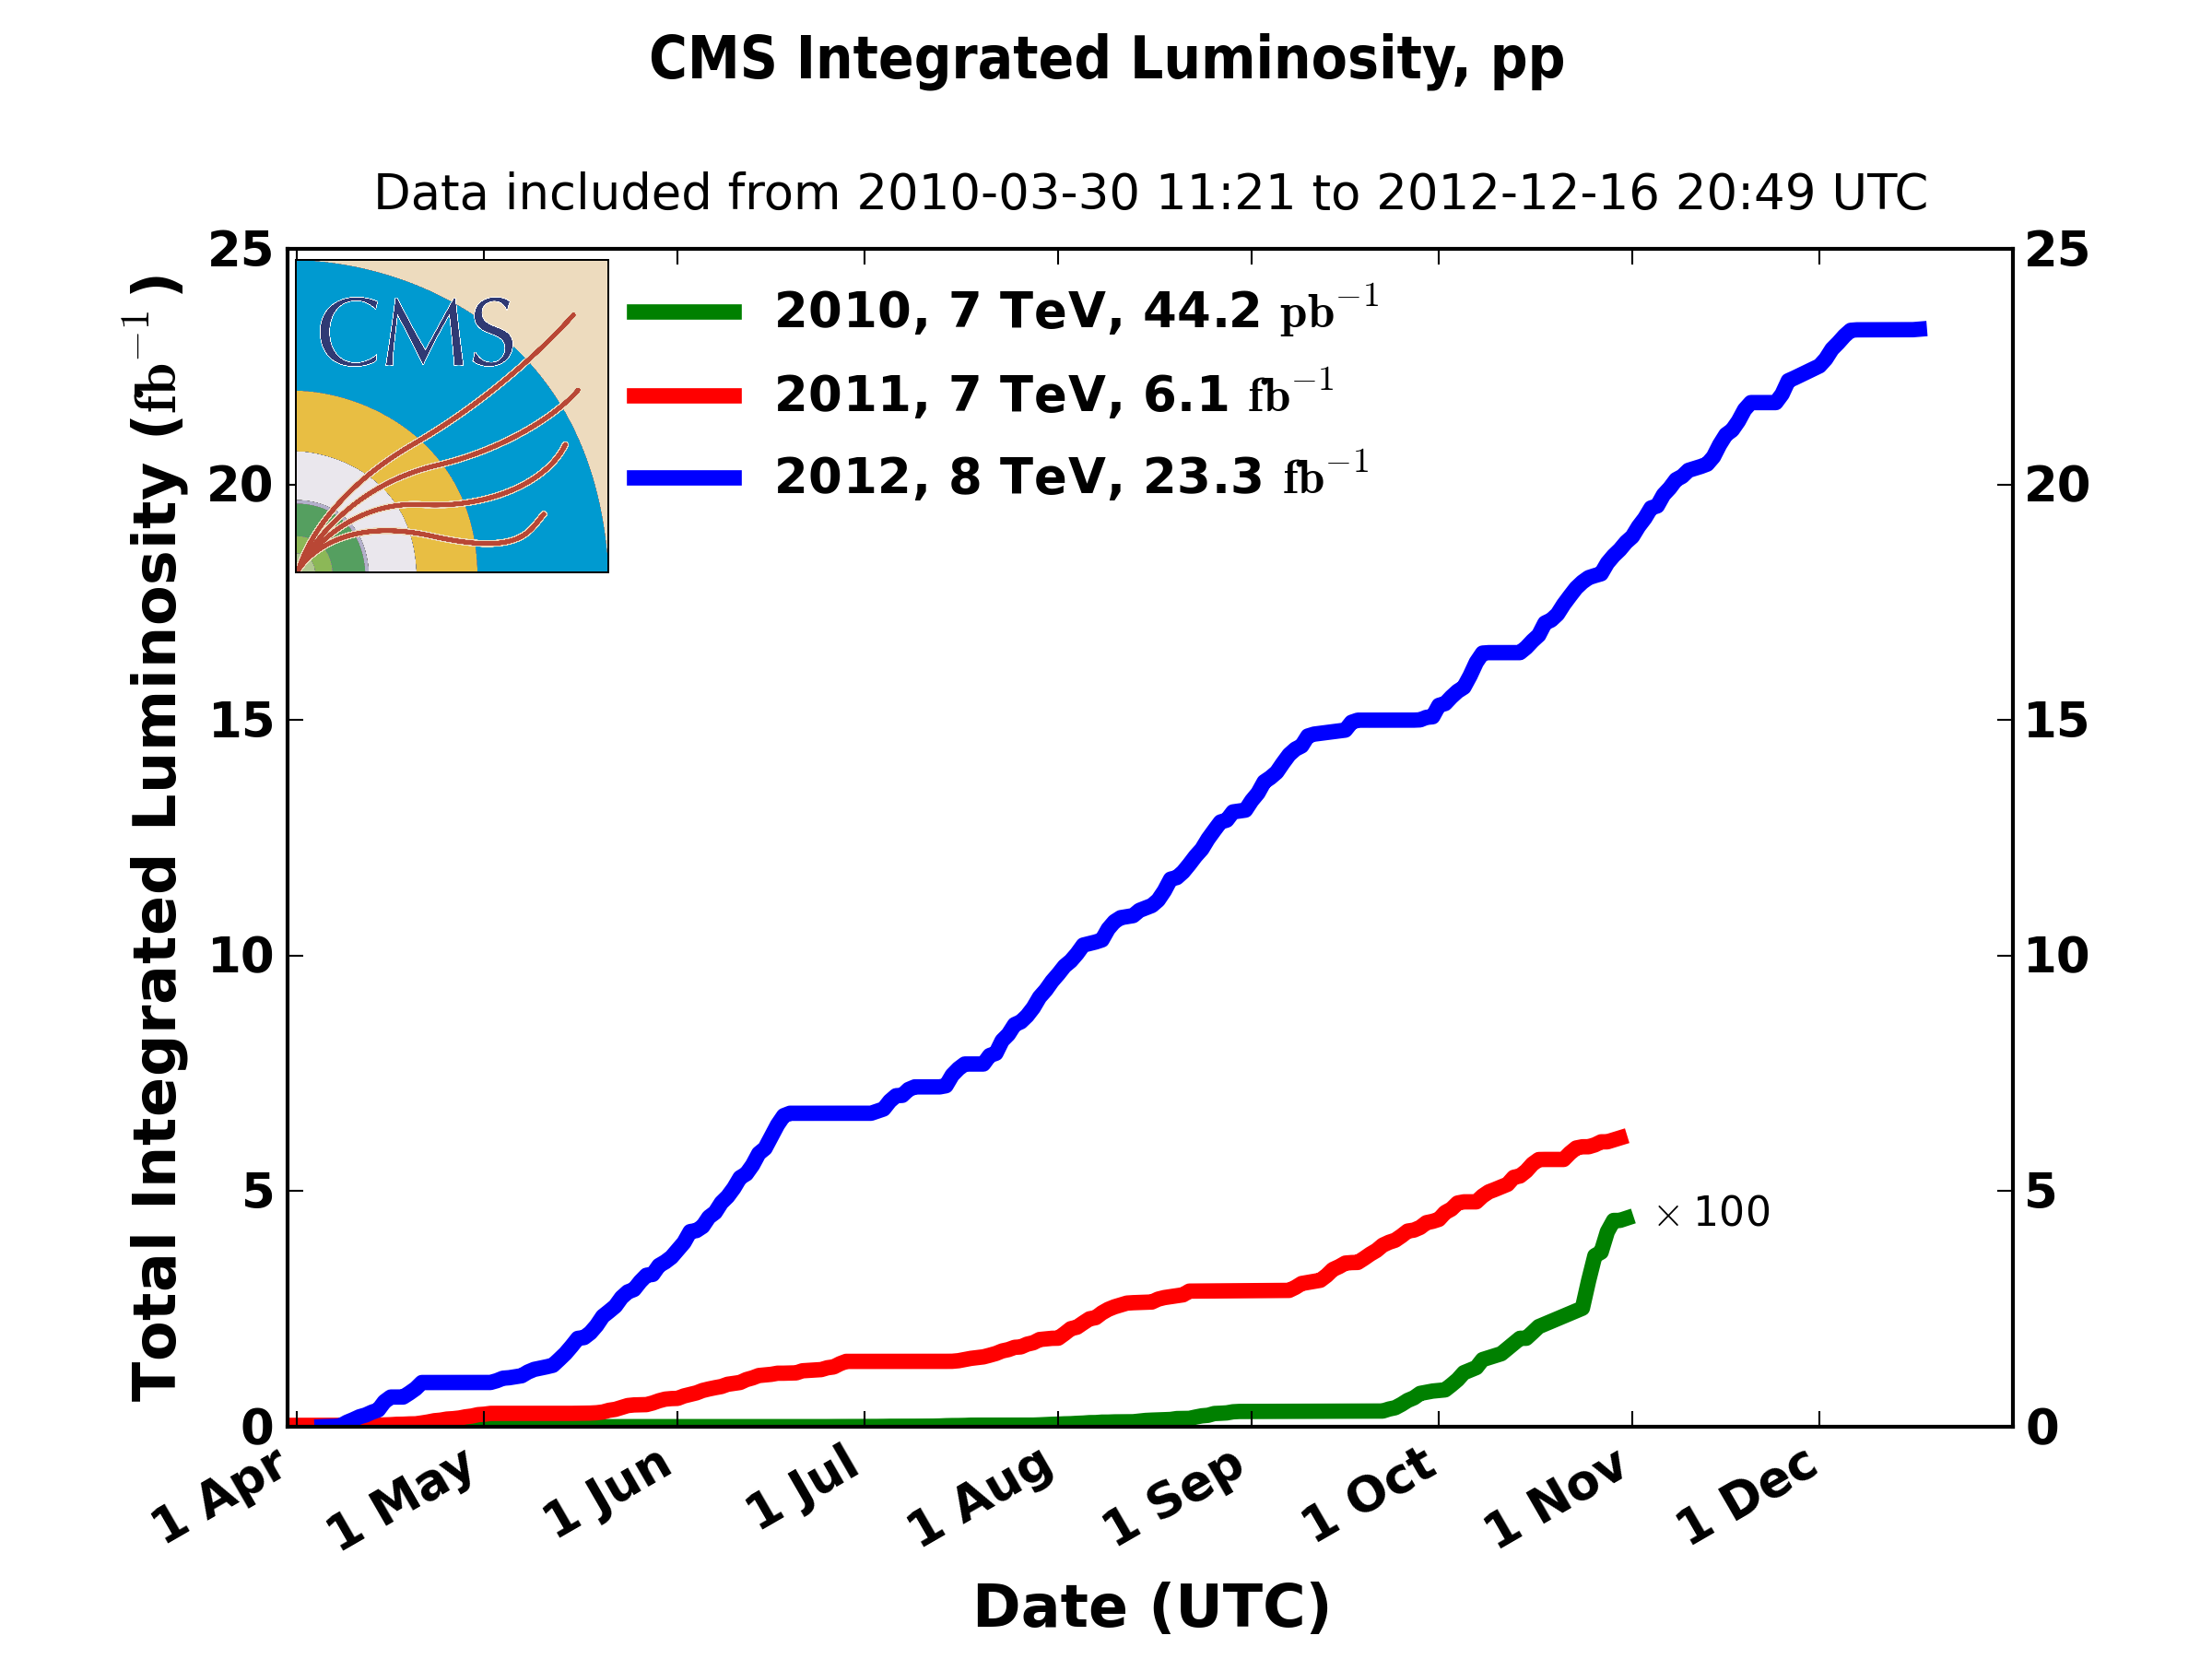
\includegraphics[width=.45\paperwidth,]{../figures/int_lumi_cumulative_pp_2.png}
\end{textblock*}
}
\subsection{CMS}
\frame{
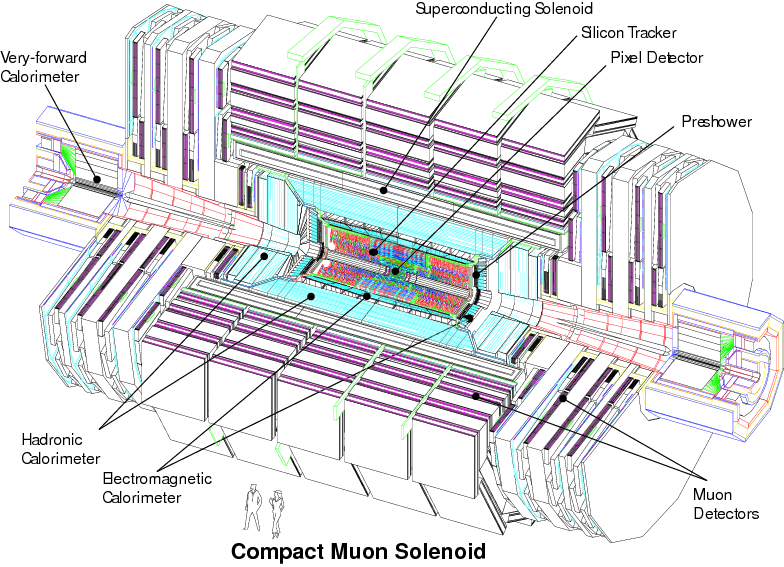
\includegraphics[width=.8\paperwidth,]{../figures/cms_complete_labelled.png}
\begin{textblock*}{5cm}(7.0cm,1.6cm) % {block width} (coords)
\visible<2>{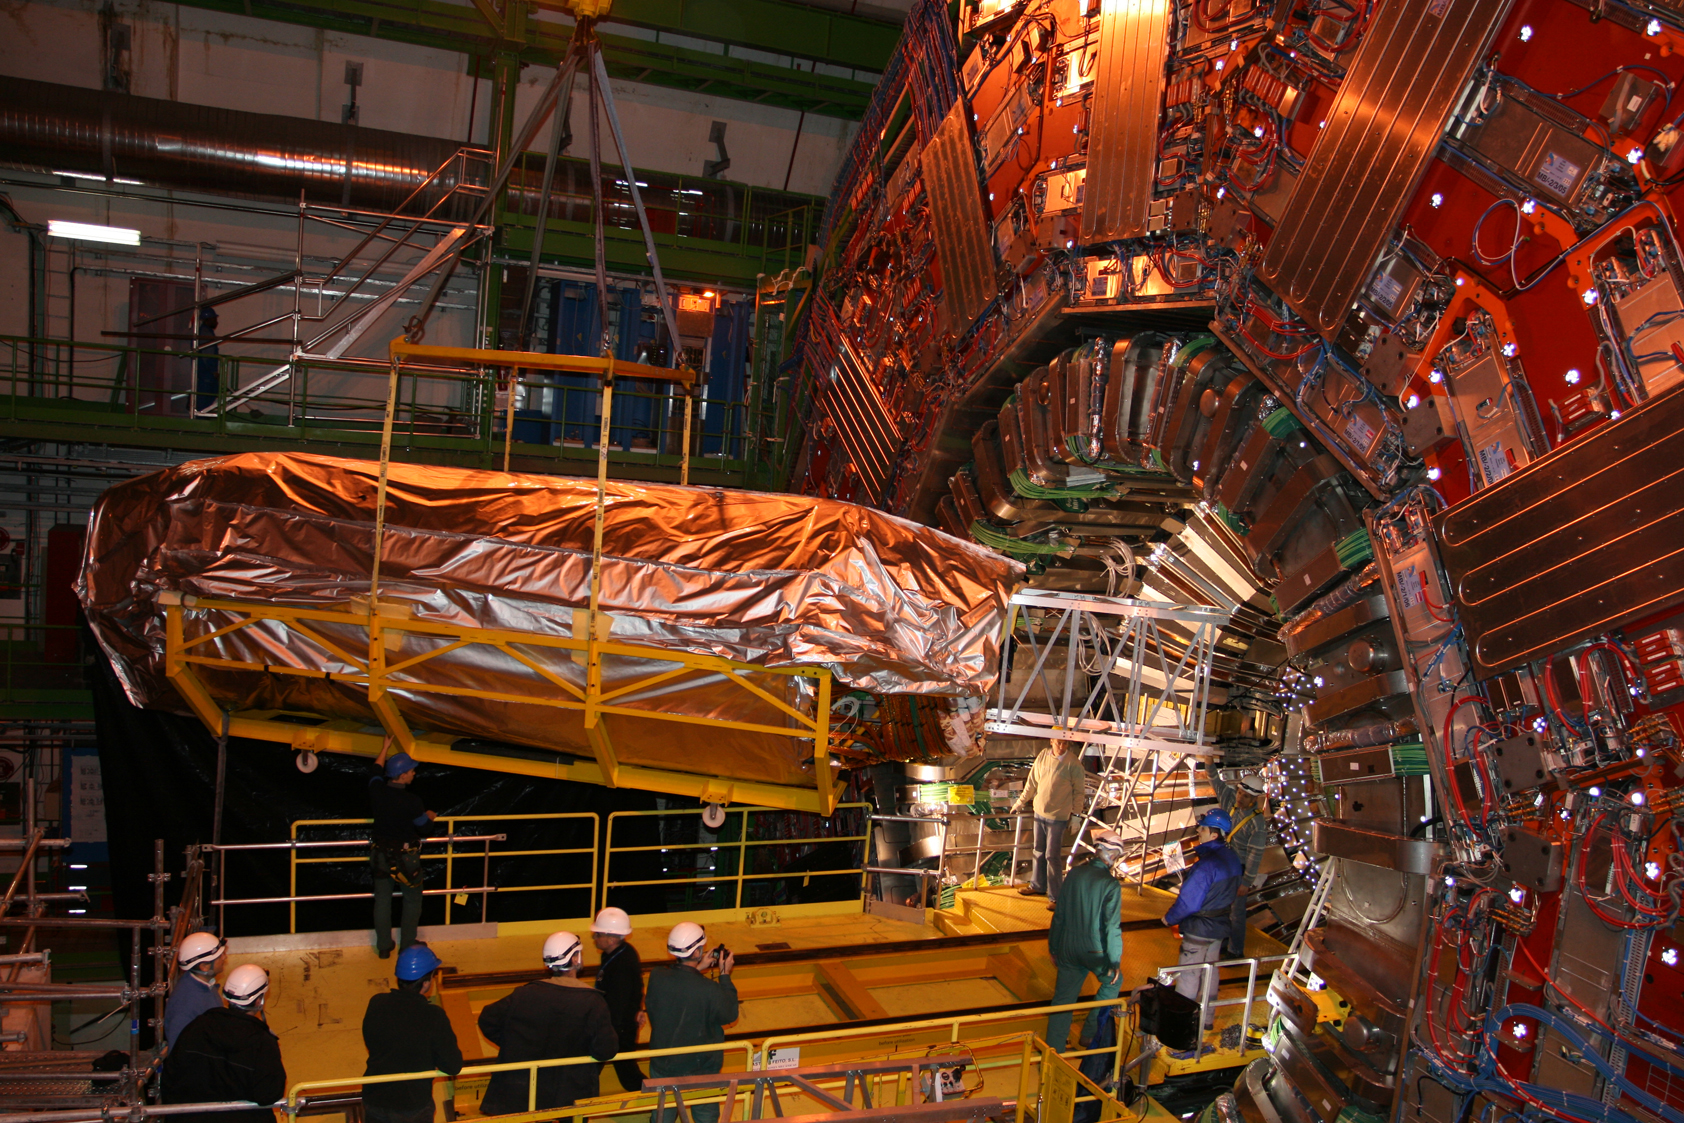
\includegraphics[width=.43\paperwidth,]{../figures/bul-pho-2008-003.jpg}}

\end{textblock*}
\begin{textblock*}{5cm}(.5cm,5.5cm) % {block width} (coords)
\visible<3>{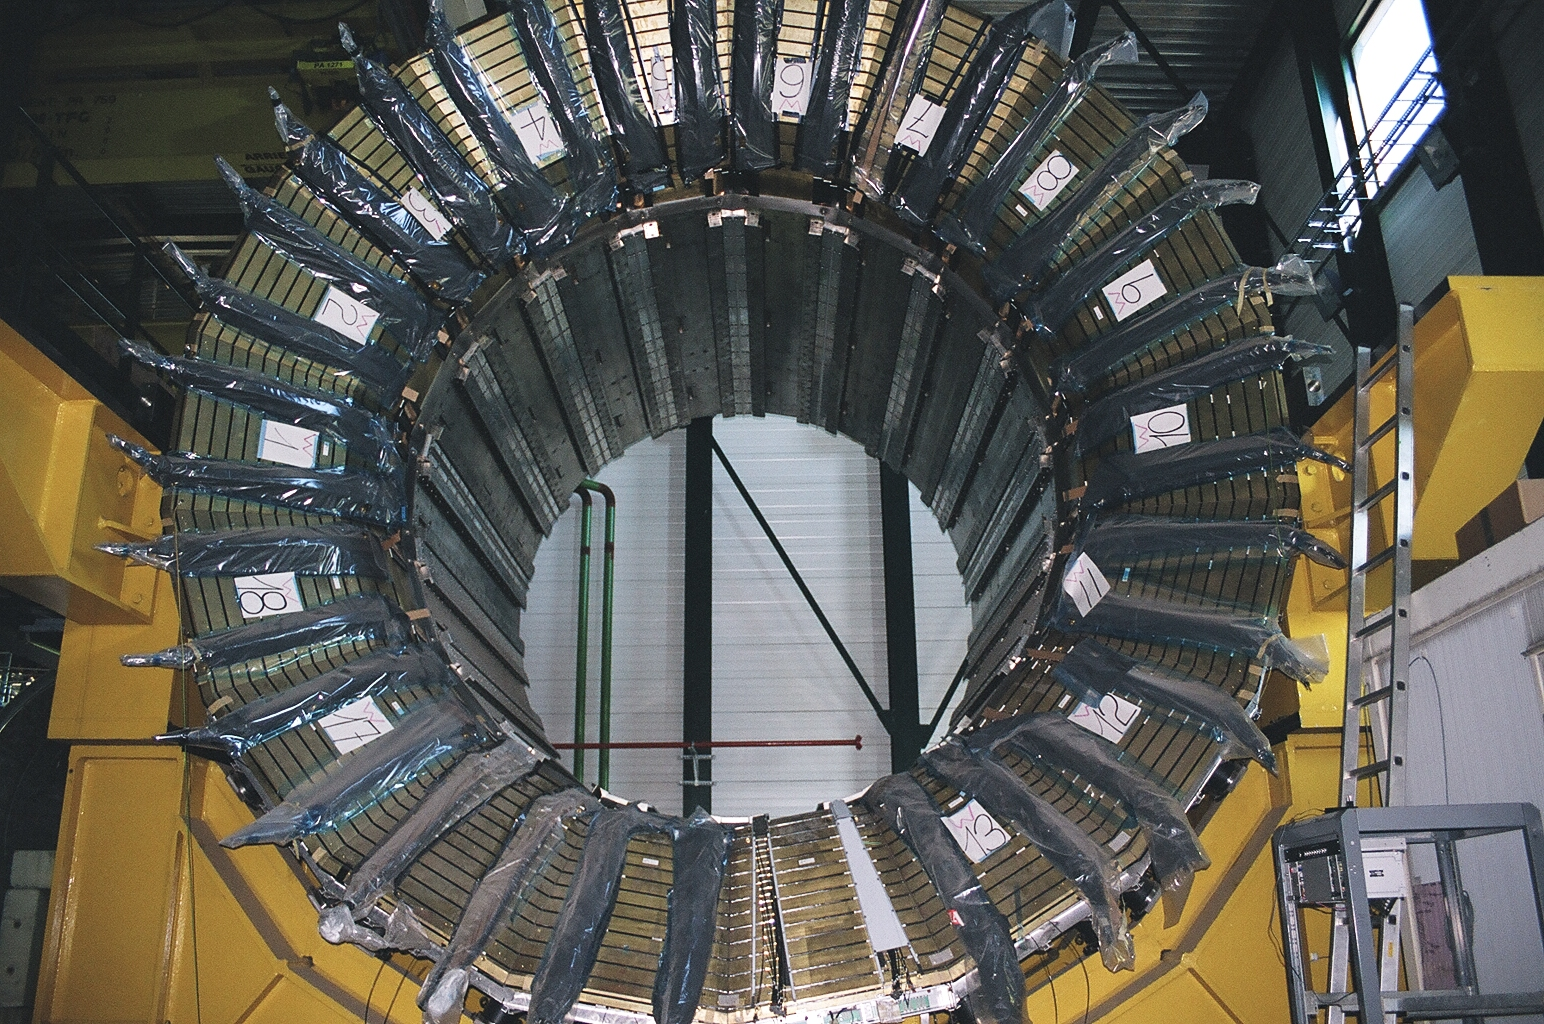
\includegraphics[width=.43\paperwidth,]{../figures/hcal-2005-001.jpg}}\par
\end{textblock*}


\begin{textblock*}{5cm}(3.0cm,3.0cm) % {block width} (coords)
\visible<4>{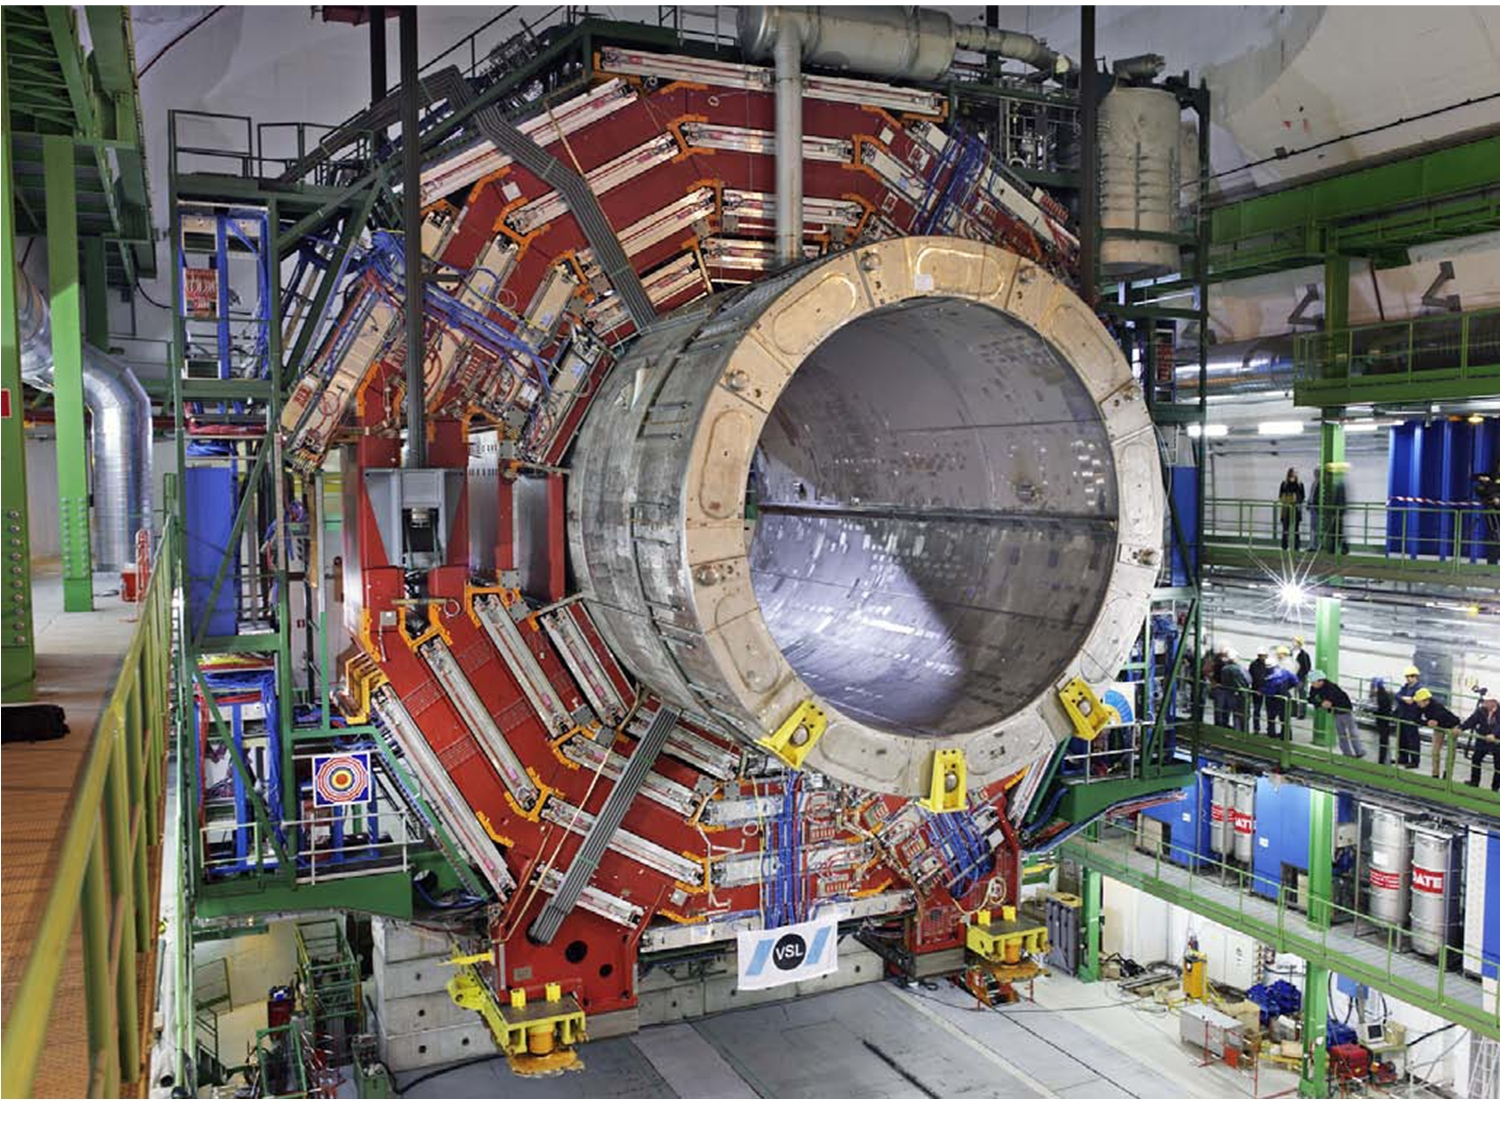
\includegraphics[width=.43\paperwidth,]{../figures/3011_1.jpg}}\par
\end{textblock*}

\begin{textblock*}{5cm}(7.1cm,4.0cm) % {block width} (coords)
\visible<5>{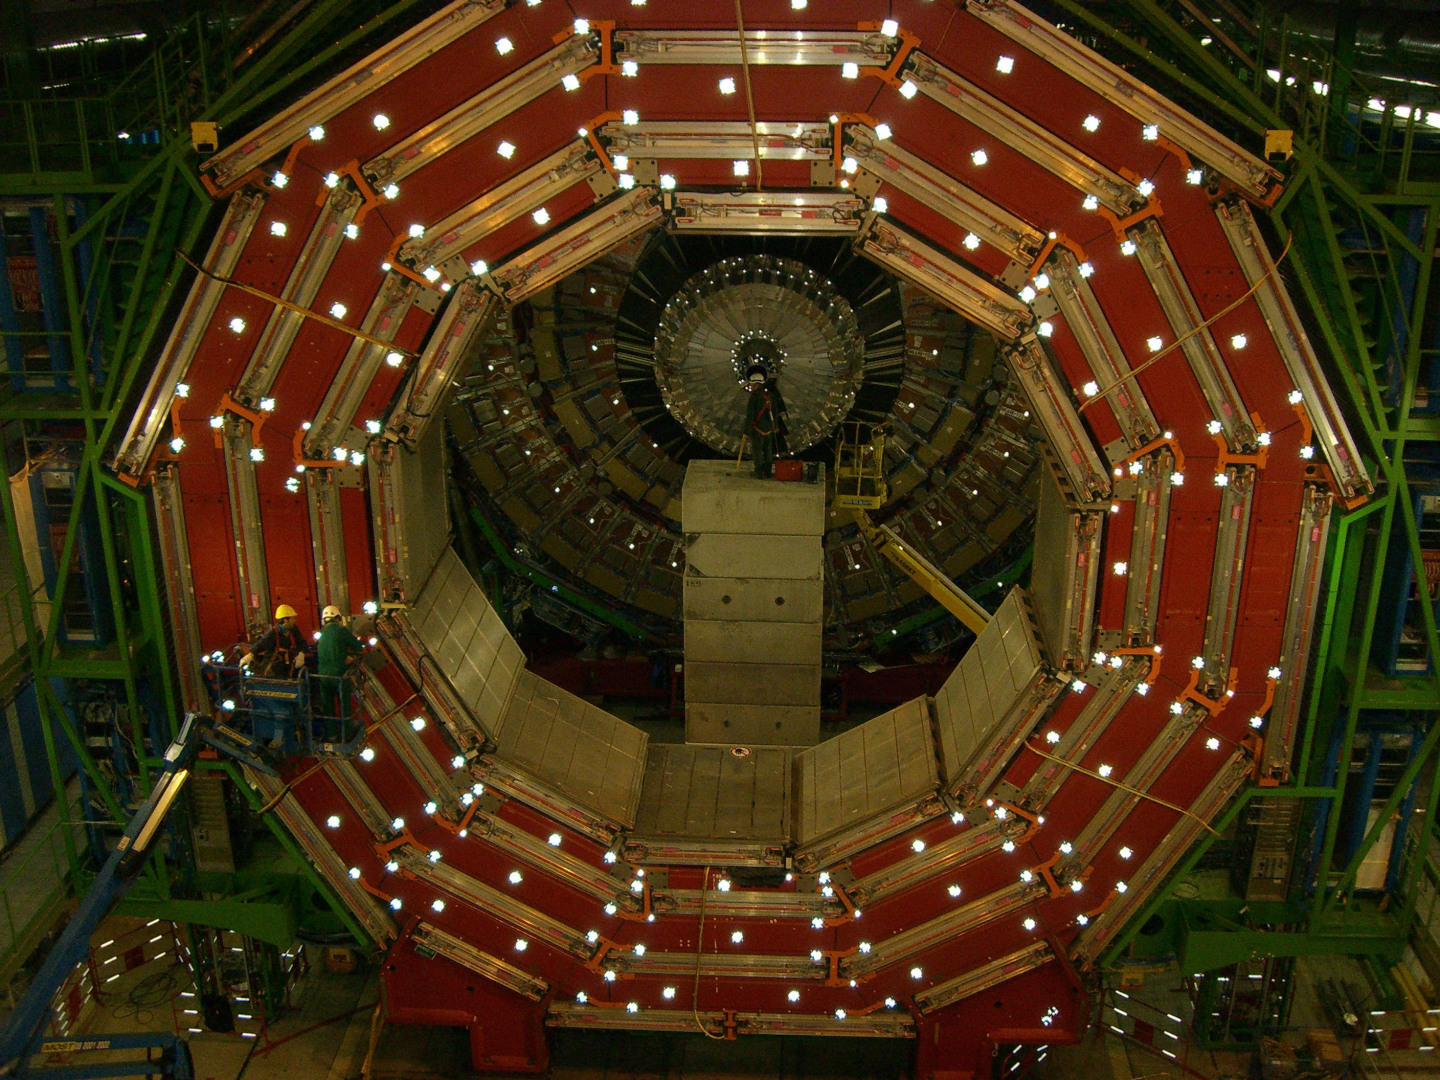
\includegraphics[width=.43\paperwidth,]{../figures/oreach-2007-001_09.jpg}}\par
\end{textblock*}

}
\frame{
\frametitle{A Slice of CMS}
\begin{textblock*}{5cm}(.5cm,2cm) % {block width} (coords)
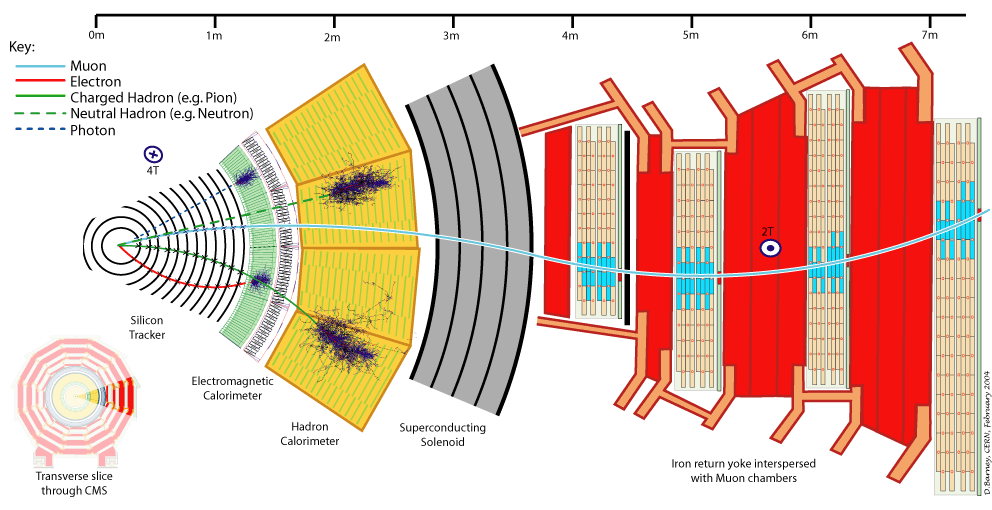
\includegraphics[width=.9\paperwidth,]{../figures/CMS_Slice.png}
\end{textblock*}
}

\frame{
\frametitle{The Coordinate System}
\begin{center}
\includegraphics[width=.48\paperwidth,]{../figures/Figures_T_Coordinate.png}
\includegraphics[width=.28\paperwidth,]{../figures/Pseudorapidity2.png}

\end{center}
\small{
Azymuthal angle ($\phi$): angle around beam line\\
Known and conserved quantities: 
\begin{itemize}
\item transverse momentum, $\pt \equiv P \sin\theta$
\item transverse energy, $E_{T} \equiv E \sin\theta$
\end{itemize}
$0 \leq \theta \leq \pi$ where $\theta$ is the polar angle from the beam-line; 


\begin{itemize}
\item pseudo-rapidity:
\begin{equation*}
        \eta \equiv −\ln\left( \tan\left(\theta/2\right)\right)
        \label{pseudo}      
\end{equation*}

\end{itemize}
}

}
%%
\section{Search Strategy}
\subsection{Models}
\frame{
\frametitle{Search Stategy}

\color{black}{Early searches at LHC focused on \\high cross section production \\models $\rightarrow$ $\frac{\sigma\left(\tilde{g}\tilde{g}\right)}{\sigma\left(\tilde{t}\tilde{t}\right)} \sim 100$.}
~\\
~\\
Current situation: \\
gluino masses $<1.1~TeV$ and $1^{st}$- \\and 
$2^{nd}$-generation squark masses \\ $<800~GeV$ are excluded 
\\
~\\
~\\
~\\
One expects relatively light top, $<1~TeV$, if SUSY 
is to be the natural solution to the hierarchy problem 

\begin{textblock*}{10cm}(10cm,4.2cm) % {block width} (coords)
\color{red!80}{$\tilde{g}\tilde{g}$}
\end{textblock*}
\begin{textblock*}{10cm}(10cm,3.2cm) % {block width} (coords)
\color{green!80}{$\tilde{q}\tilde{q}$}
\end{textblock*}
\begin{textblock*}{10cm}(10.6cm,5.0cm) % {block width} (coords)
\color{blue!80}{$\tilde{t}\tilde{t}^*$}
\end{textblock*}

\begin{textblock*}{6cm}(7.2cm,2cm) % {block width} (coords)
\includegraphics[width=0.9\textwidth, trim = .6cm .1cm .54cm .1cm, clip=true]{../figures/nlonll_lhc8_tpformat.eps}
\end{textblock*}
\begin{textblock*}{10cm}(8.41cm,2.5cm) % {block width} (coords)
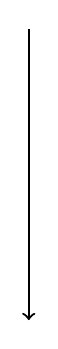
\begin{tikzpicture}
\draw [->, thick] (0,0) -- (0,-3.7);
\end{tikzpicture}
\color{black}{~\\80k gluino pairs,\\2000 stops in 20$fb^{-1}$}
\end{textblock*}
}

\section{Search Strategy}
\subsection{Models}
\frame{
\frametitle{Search Stategy}

Early searches at LHC focused on high cross section production models $\rightarrow$ $\frac{\sigma\left(\tilde{g}\tilde{g}\right)}{\sigma\left(\tilde{t}\tilde{t}\right)} \sim 100$.\\

\begin{textblock*}{10cm}(5cm,5.3cm) % {block width} (coords)
\color{red!80}{$\tilde{g}\tilde{g}$}
\end{textblock*}
\begin{textblock*}{10cm}(5cm,4.2cm) % {block width} (coords)
\color{green!80}{$\tilde{q}\tilde{q}$}
\end{textblock*}
\begin{textblock*}{10cm}(5.6cm,6.4cm) % {block width} (coords)
\color{blue!80}{$\tilde{t}\tilde{t}^*$}
\end{textblock*}
\begin{center}
\includegraphics[width=0.7\textwidth, trim = .6cm .1cm .54cm .1cm, clip=true]{../figures/nlonll_lhc8_tpformat.eps}
\end{center}
\begin{textblock*}{10cm}(4.31cm,4.0cm) % {block width} (coords)
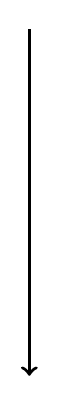
\begin{tikzpicture}
\draw [->, very thick] (0,0) -- (0,-4.4);
\end{tikzpicture}
~\\80k gluino pairs,\\2000 stops in 20$fb^{-1}$
\end{textblock*}
}

\frame{
\frametitle{Search Strategy}
\color{black}
Conserved quantity, R-parity:

\begin{equation*}
\label{eq:r-par}
R = \left(-1\right)^{3B+L+2s}
\end{equation*}
\begin{center}
SM: R = +1, SUSY: R = -1. 
\end{center}

R-parity conserving SUSY theory implies:
\begin{itemize}
\item SUSY particles are pair-produced
\item a stable ``light'' supersymmetric particle (LSP). 
\end{itemize}

In this analysis: LSP is assumed to be the neuralino: $\tilde{\chi}_1^0$ \\
~\\
\begin{columns}[cc]
  \column{0.5\paperwidth}\centering
  ``T2tt''\\
  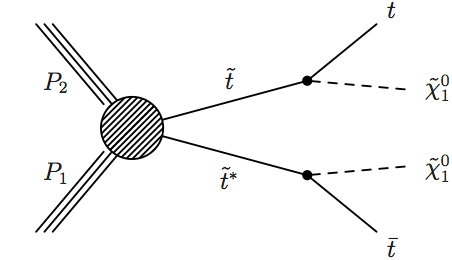
\includegraphics[width=.65\columnwidth,]{../figures/T2tt.png}
  \column{0.5\paperwidth}\centering
  ``T2cc''\\
  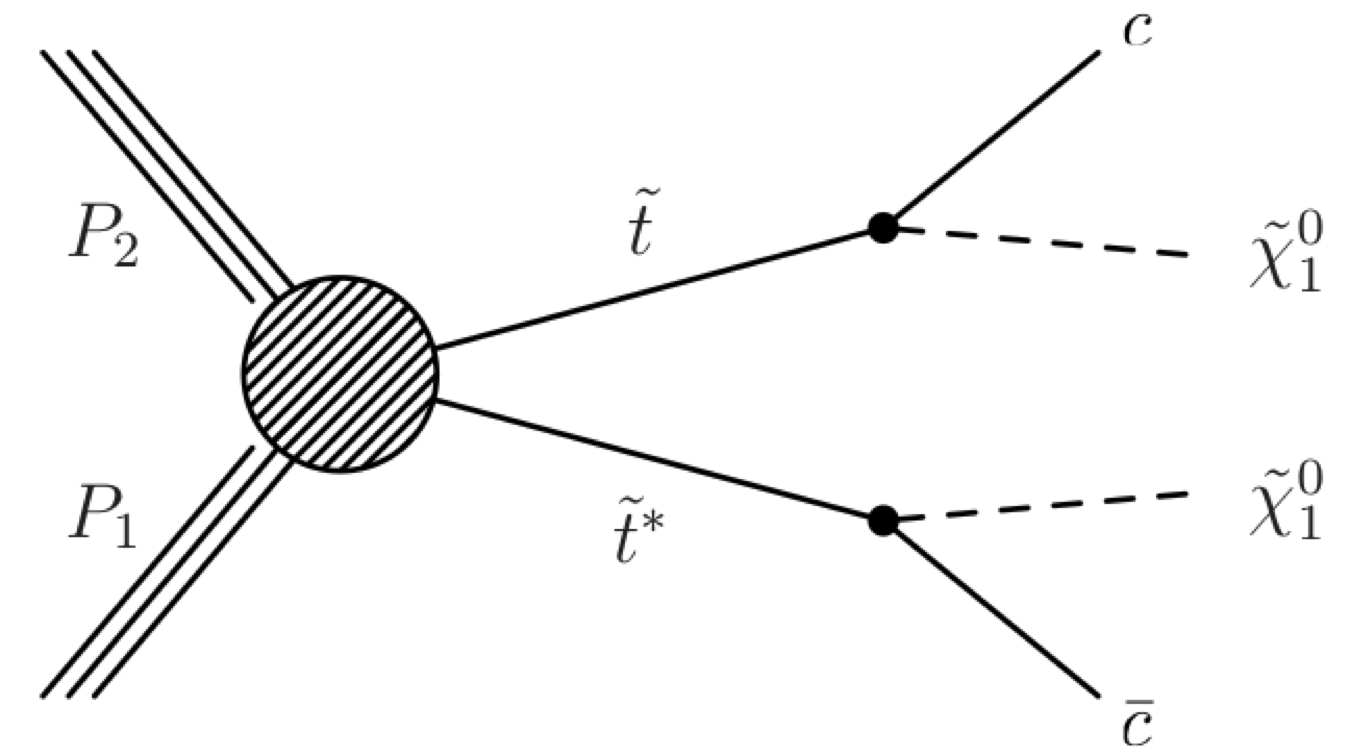
\includegraphics[width=.65\columnwidth,]{../figures/T2cc.png}
\end{columns}
}
%%
\color{black}
\frame{
\frametitle{Search strategy}
%100\% branching fraction.
~\\
``T2tt'': $\tilde{t} \rightarrow t \tilde{\chi}_1^0$
\begin{itemize}
\item highest reach for $m_{\tilde{t}}$
\end{itemize}

``T2cc'': $\tilde{t} \rightarrow c \tilde{\chi}_1^0$
\begin{itemize}
\item i.e. $\Delta M \equiv m_{\tilde{t}} - m_{\tilde{\chi}_1^0} < 80~GeV$, (mass of W) 
\item top squark can only decay to a charm quark and neutralino.
\item dependent on initial state radiation 
\end{itemize}
\begin{center}
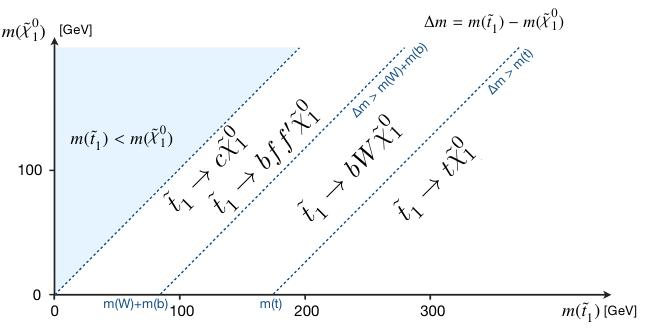
\includegraphics[width=0.55\textwidth,]{../figures/mstop_mLSP_plane.jpg}
\end{center}
final state: ``Jets'' + undetected energy
}

\frame{
\frametitle{Calorimeter Jets}
%\begin{columns}[c c]
%\column{0.5\paperwidth}
\begin{itemize}
\item ``Traditional'' jet reconstruction
\item Calorimeter towers 
  \begin{itemize}
    \item 1 HCAL cell $\sim 0.1$ ($\Delta \phi \times \Delta \eta$)
    \item 25 ECAL crystals $\sim 0.01$ ($\Delta \phi \times \Delta \eta$)
  \end{itemize}
\end{itemize}
\begin{center}
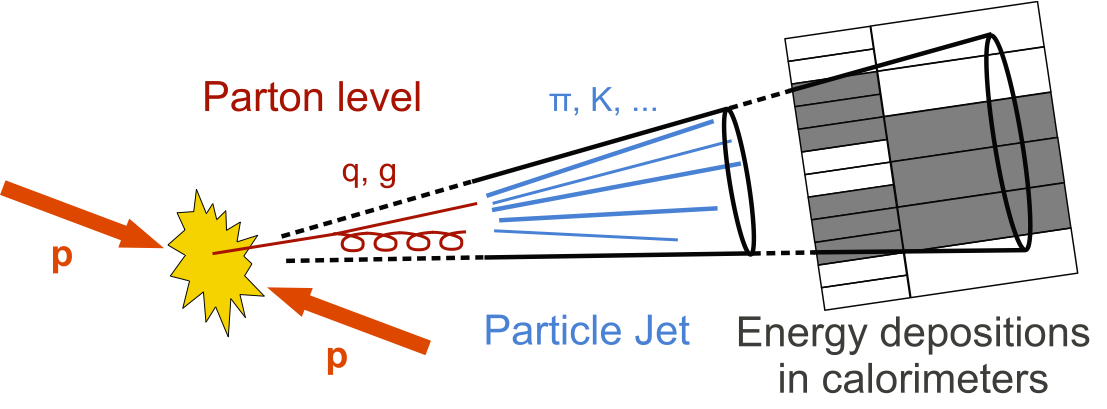
\includegraphics[width = 0.5\columnwidth]{../figures/Sketch_PartonParticleCaloJet.png}
\end{center}
\begin{itemize}
\item Does not make use of ECAL granularity 

\item Jet resolution driven by HCAL: 
  \begin{itemize}
  \item HCAL resolution $\sim 100\%/\sqrt E $
  \item non-compensating $\rightarrow$ non-linear response 
  \end{itemize}
\item Low $p_{T}$ charged hadrons bent outside jet
\end{itemize}
%\column{0.5\paperwidth}


%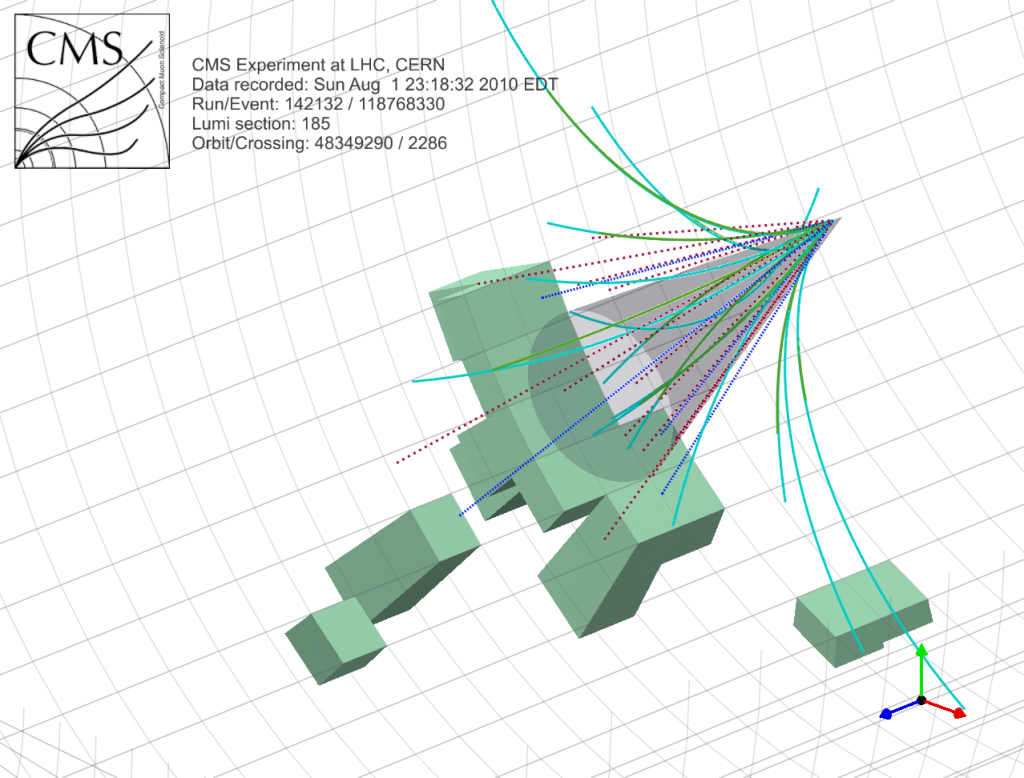
\includegraphics[width = 1.0\columnwidth]{../figures/JetConeWithTracks.png}
%\end{columns}
}
\frame{
\frametitle{Particle Flow Jets}
\begin{columns}[c c]
\column{0.5\paperwidth}
Particle Flow (PF) reconstructs all stable particle in the event: $h^\pm$, $\gamma$, $h^0$, $e$, $\mu$
\begin{itemize}

\item On average jets are: 
\item $\sim65\%$ charged hadrons, $\sim25\%$ photons, $\sim10\%$ neutral hadrons 
\item Using the silicon tracker (vs. HCAL) to measure charged hadrons 
  \begin{itemize}
  \item Improves resolution, avoids non-linearity 
  \item Decreases sensitivity to the fragmentation pattern of jets 
  \end{itemize}
\end{itemize}
\column{0.4\paperwidth}
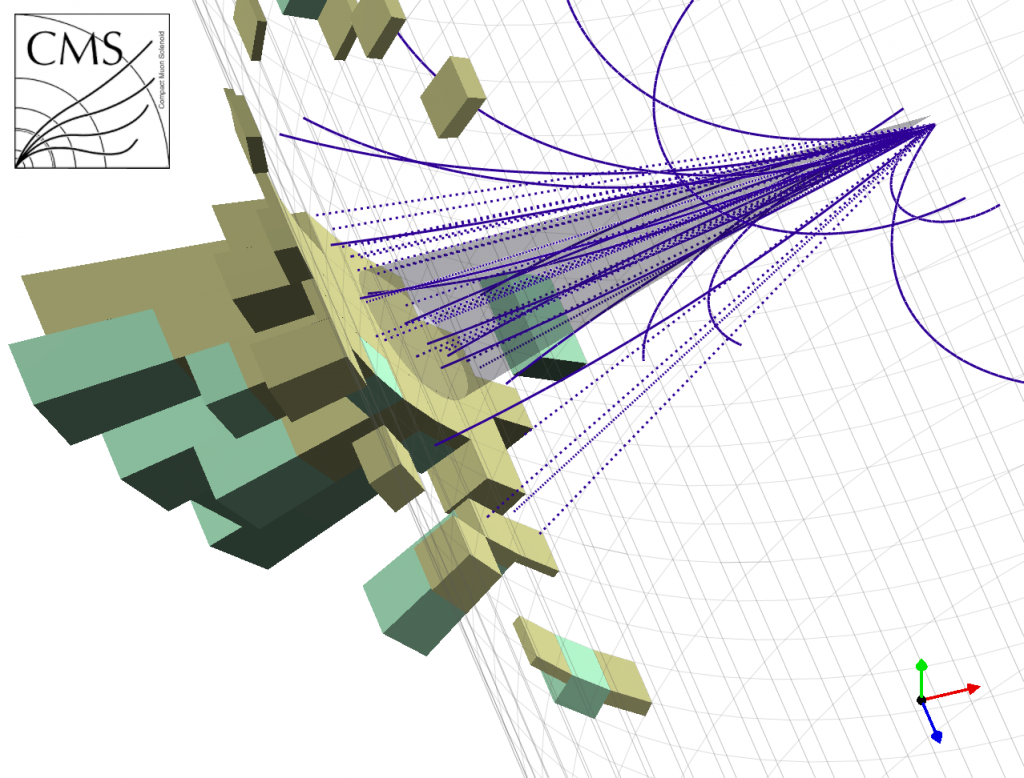
\includegraphics[width = 1.0\columnwidth]{../figures/JetConeAndPFJet.png}
\end{columns}
}

\frame{
\frametitle{Jet Resolution}
\begin{figure}[h!]
  \begin{center}
  \subfigure[]{
      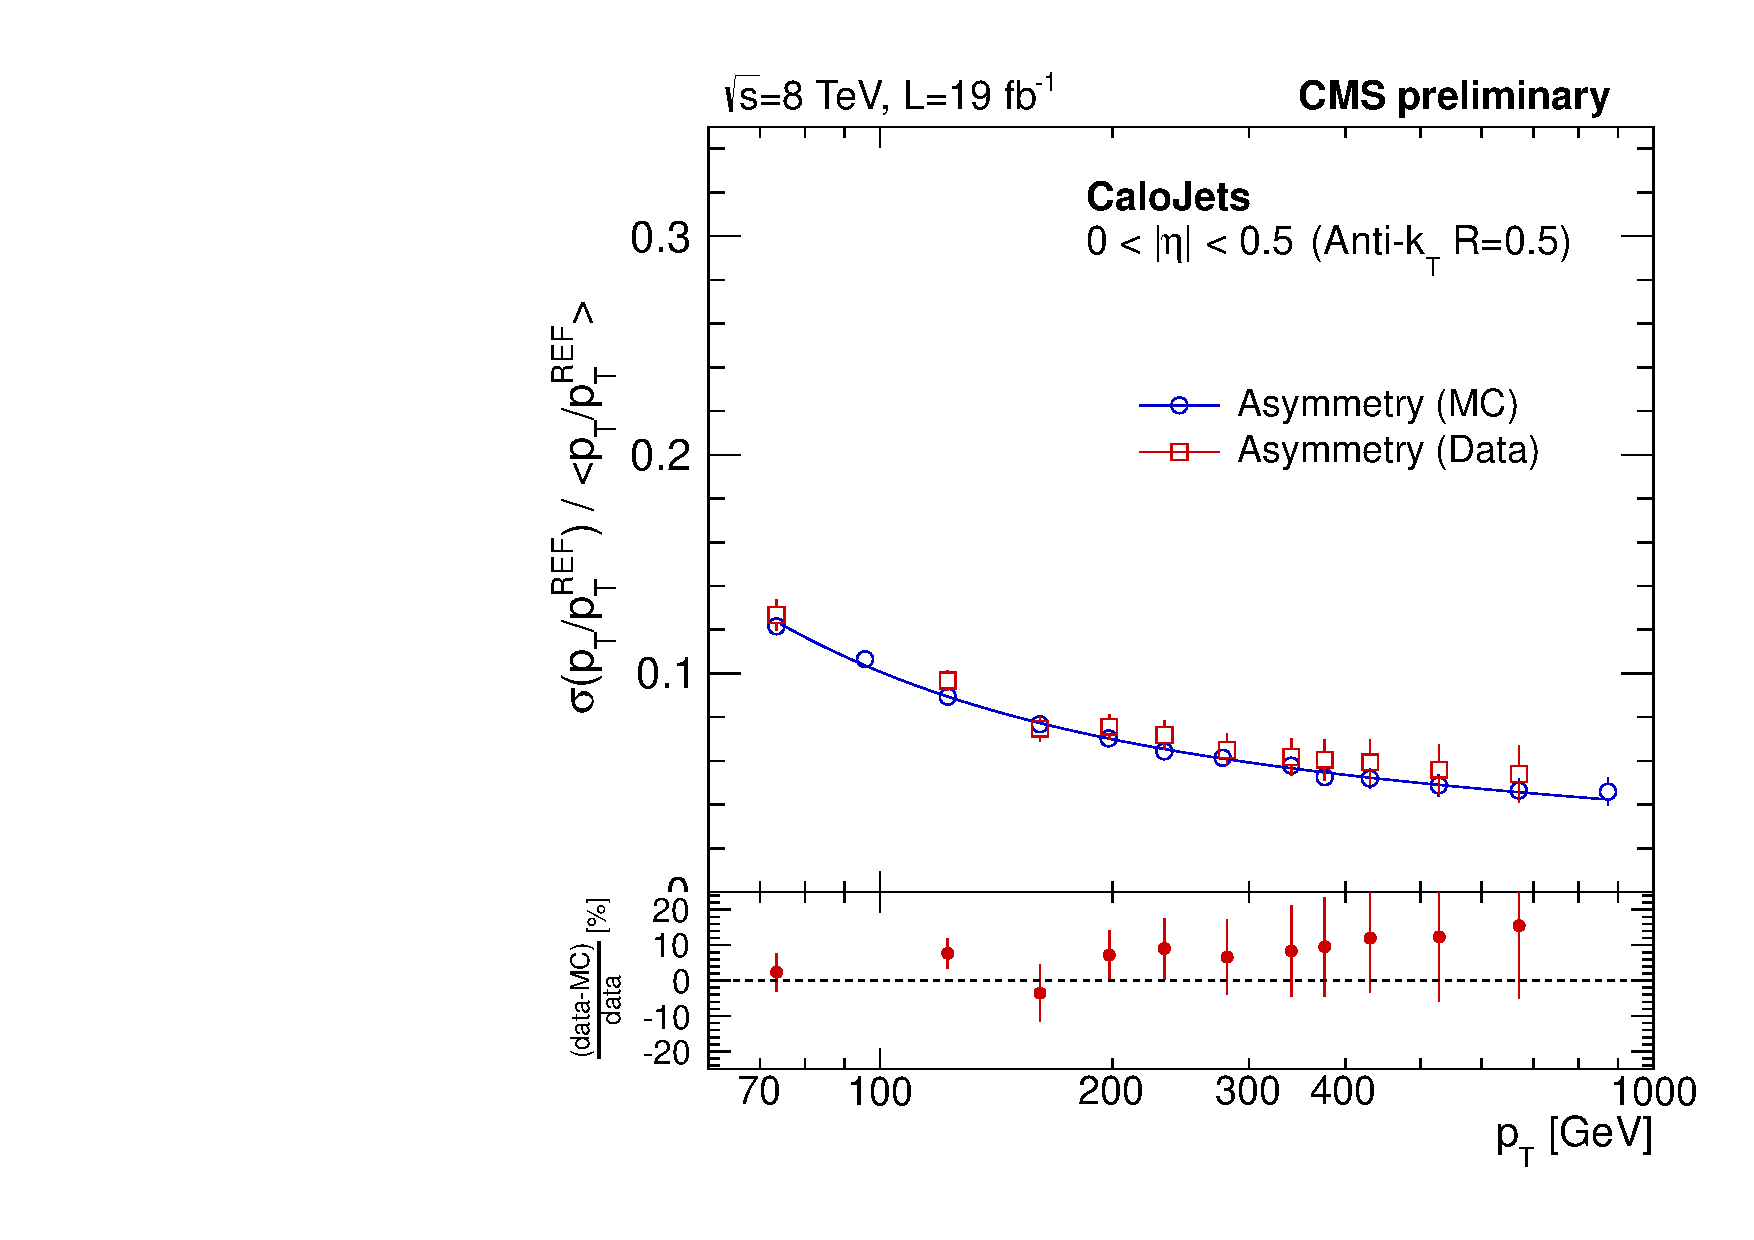
\includegraphics[width=0.45\textwidth,]{../figures/ak5calo_relRes}}
      \subfigure[]{
      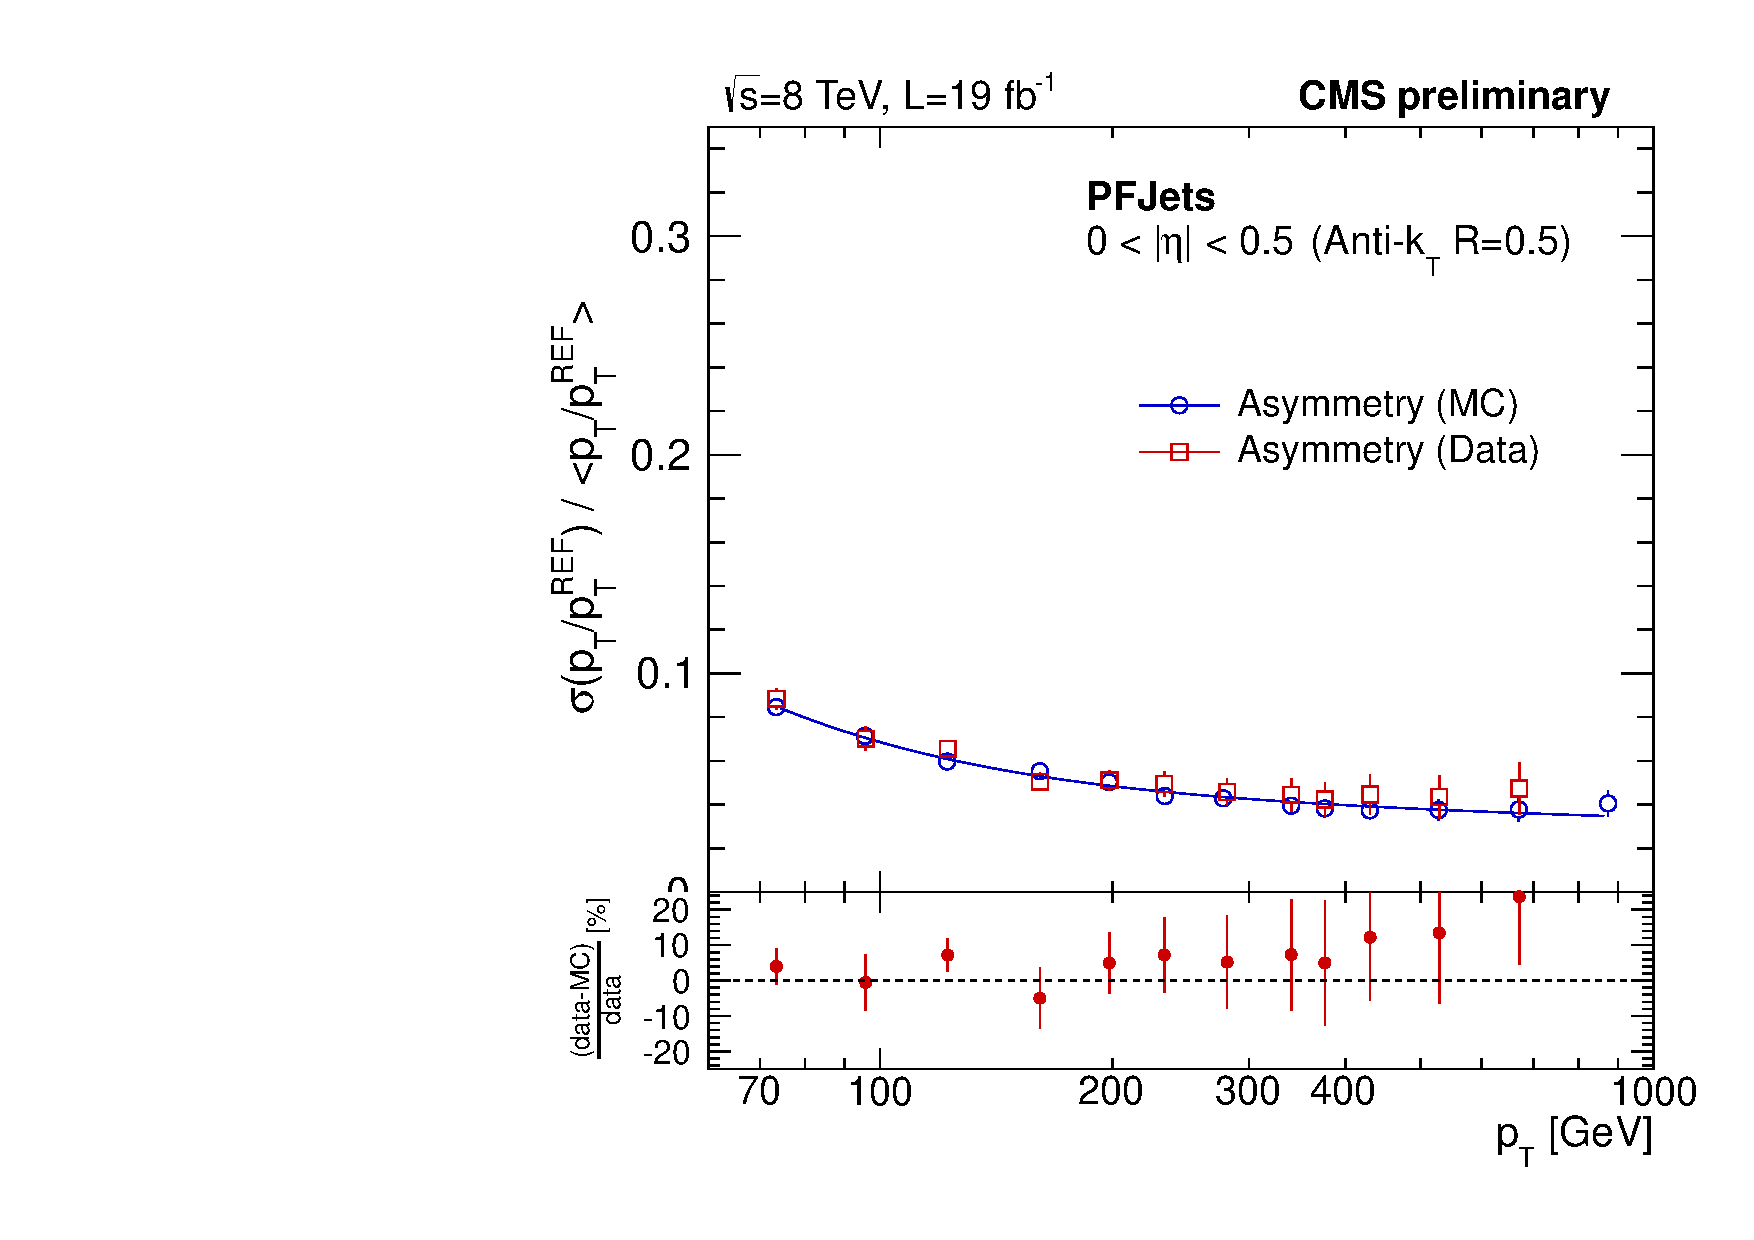
\includegraphics[width=0.45\textwidth,]{../figures/ak5pf_relRes}}
      \caption{\label{fig:jetRes} The relative $\pt$ resolution as a function of jet $\pt$
              for calo jets (a) and PF jets (b) in the center of the barrel using the dijet
              $\pt$-asymmetry method.}
  \end{center}
\end{figure}
}


{
\usebackgroundtemplate{{\transparent{0.2}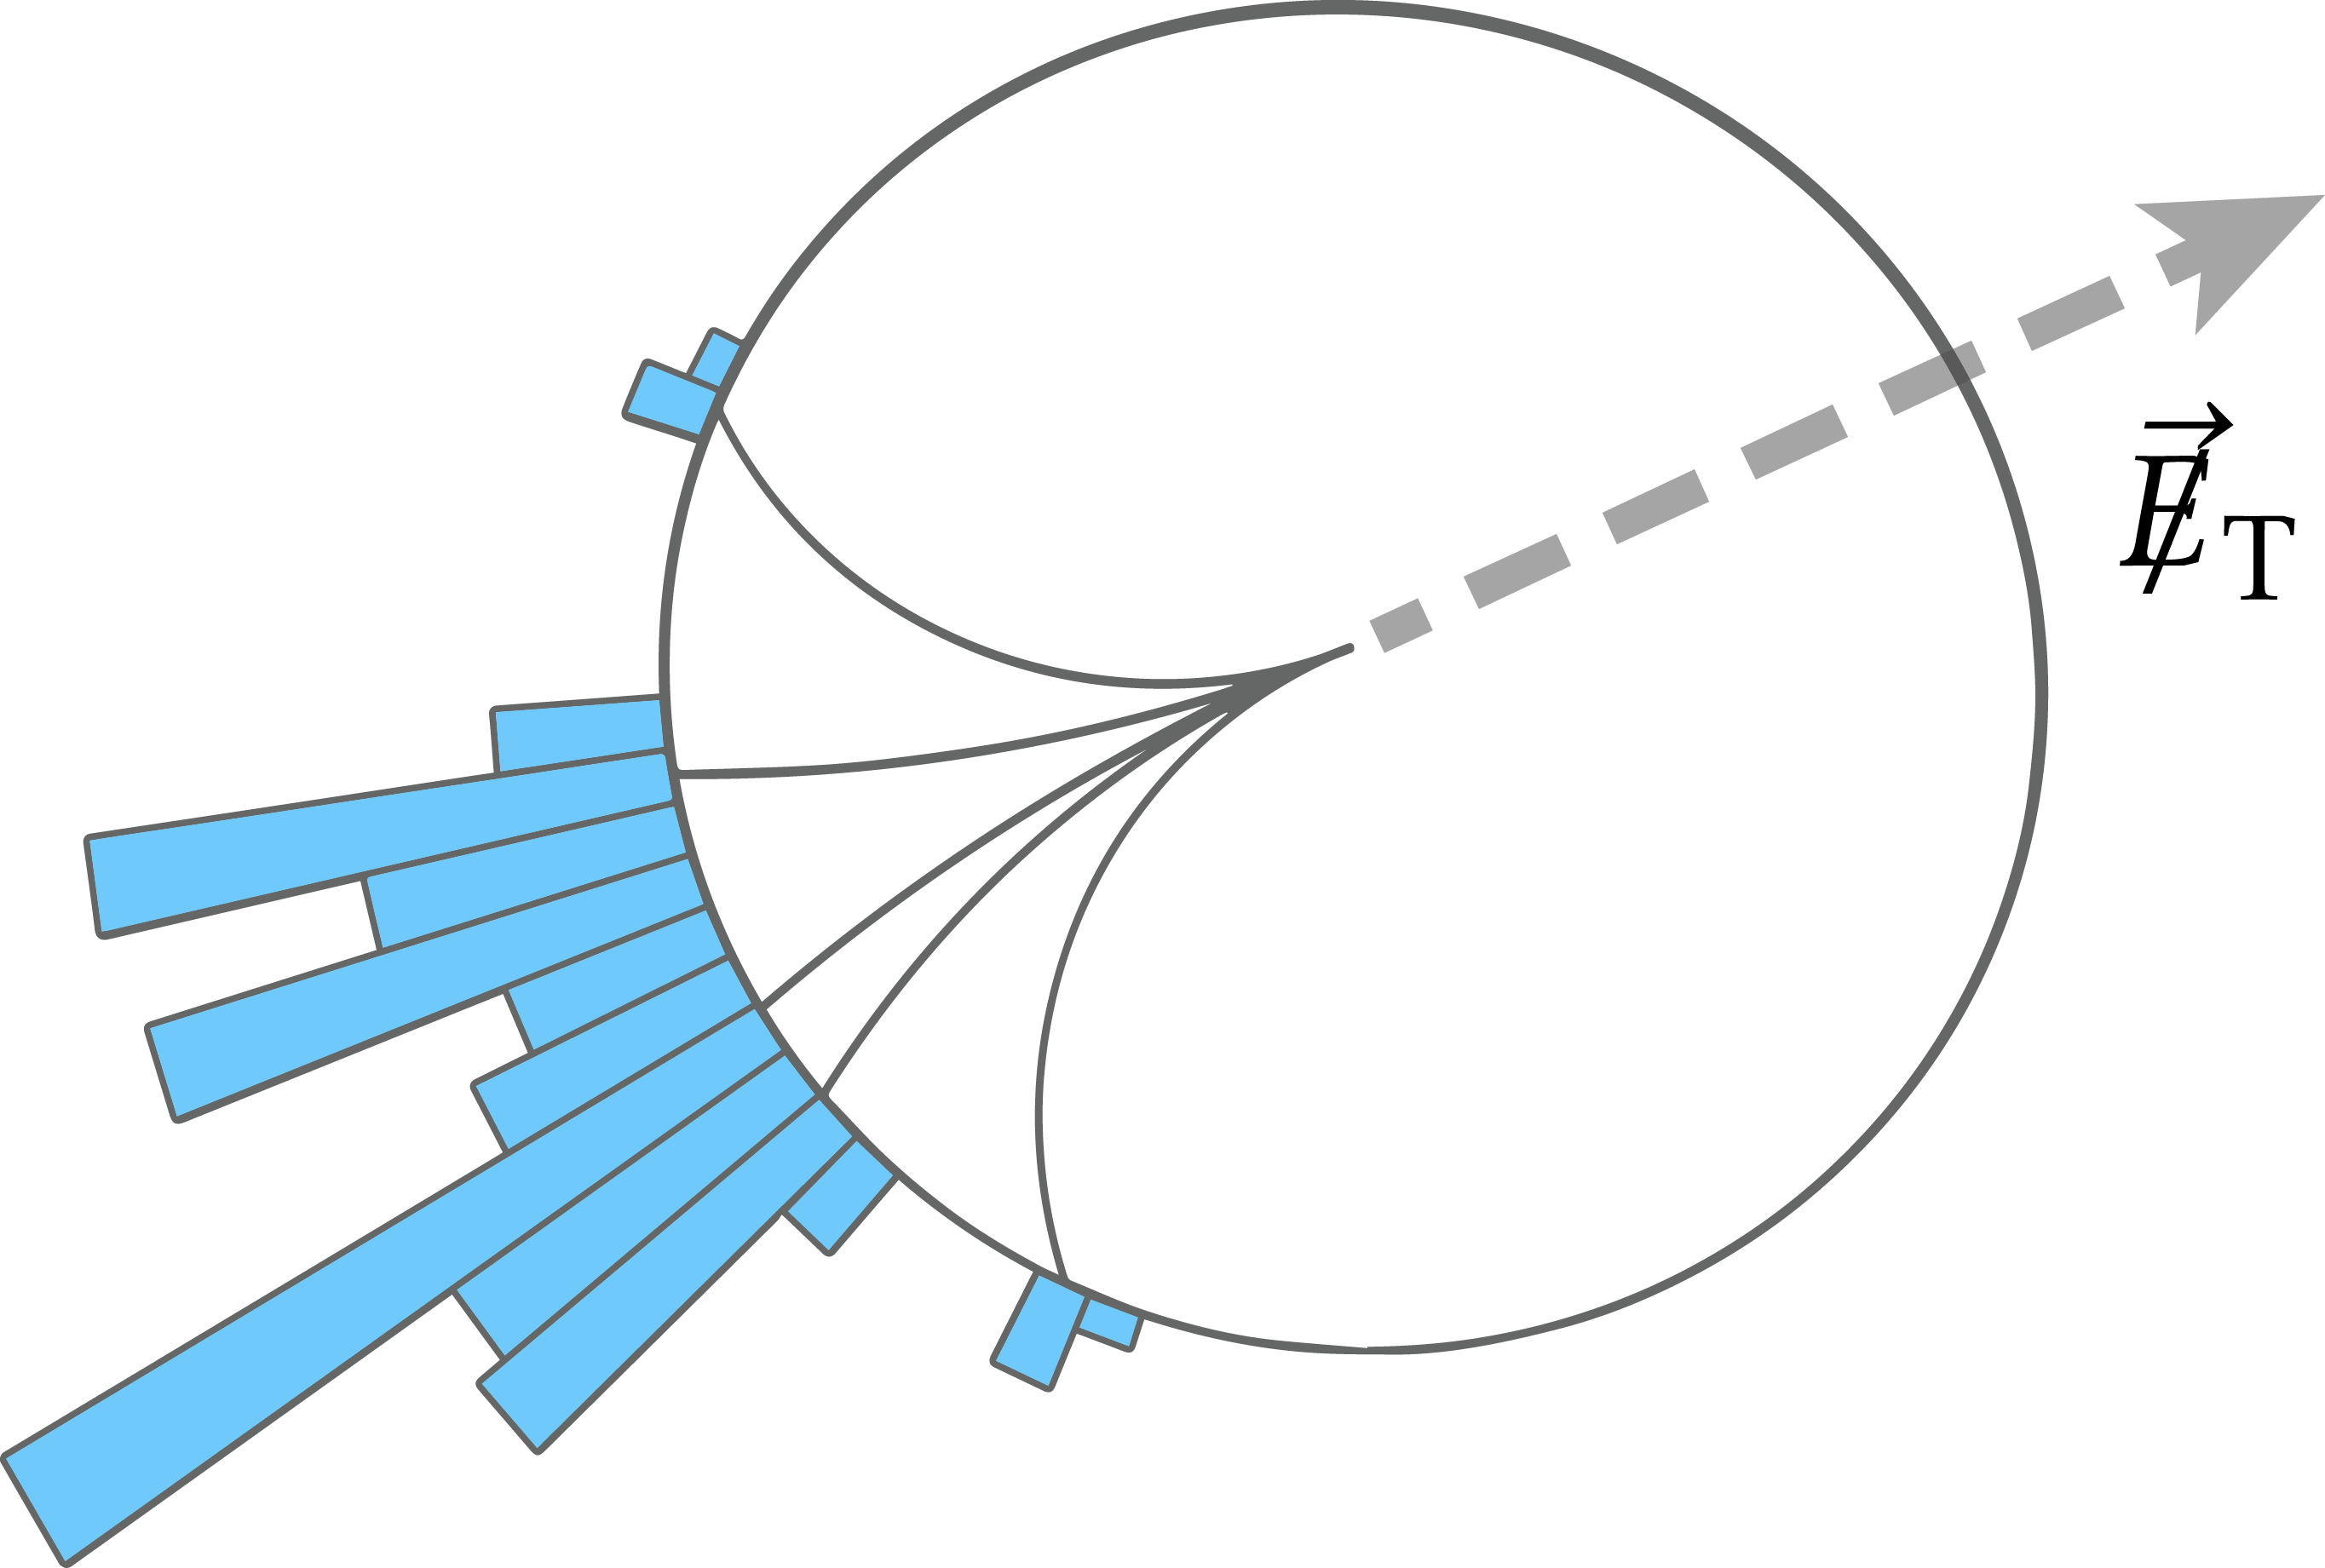
\includegraphics[width=\paperwidth,height=\paperheight]{../figures/met_schematic.png}}}
\frame{

\frametitle{Summary of Signal Characteritics}

\color{black}
\begin{itemize}
\setlength{\itemsep}{20pt}
\item Signficant hadronic content:
\begin{center}
$\scalht = \sum\limits_{j} \Et^j$
\end{center}
\item missing transverse energy: 
\begin{center}
$\mht$ =$\sum\limits_{j} \vec{\Et}^j$ , $\met = \sum\limits_{\texttt{all objects}} \Et^j$ 
\end{center}
\item no leptons
\item T2tt $\rightarrow$ b-quarks
\end{itemize}
}


}

\subsection{backgrounds}

\frame{
\frametitle{Backgrounds}
\begin{columns}[cc]
\column{0.3\paperwidth}\centering
~\\
\wj; \wlnu\\
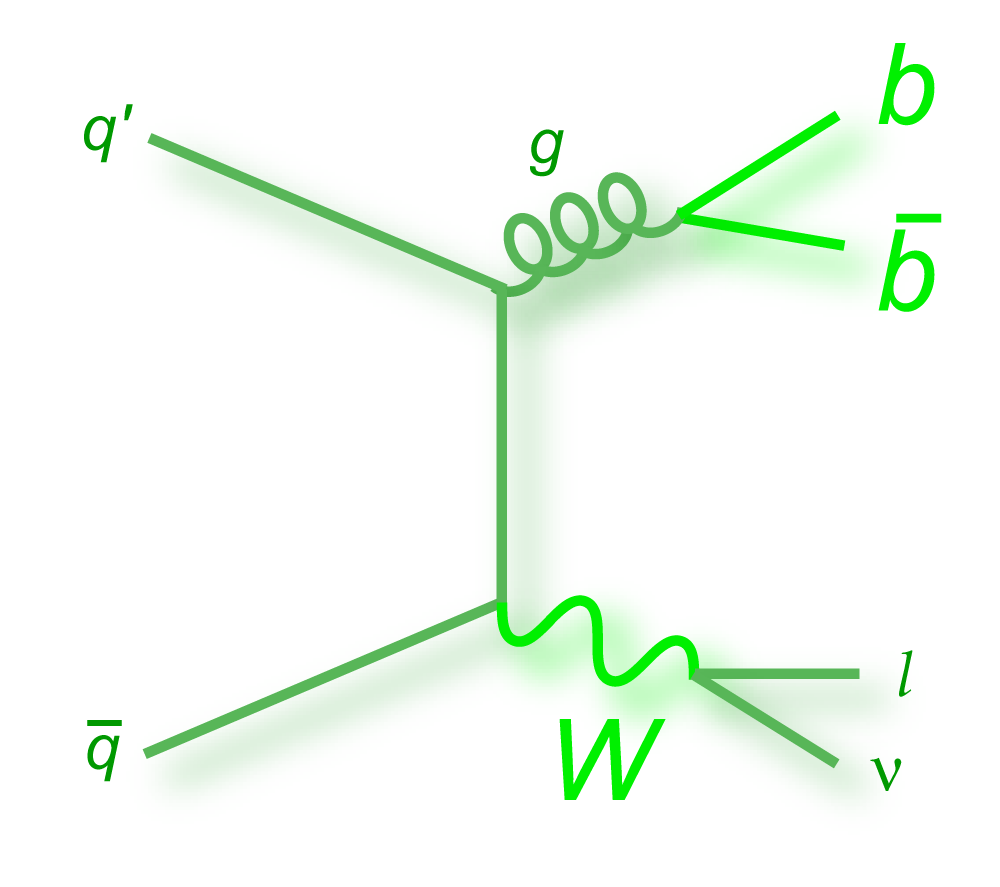
\includegraphics[height = 0.3\paperheight]{../figures/feynman/feynman_Wbb_ljets_green.png}\\
~\\
~\\
\zj; \znunu\\
\includegraphics[height = 0.3\paperheight]{../figures/feynman/feynman_Z_llbb_bold_khaki.png}
%\column{0.3\paperwidth}\centering
\column{0.7\paperwidth}\centering
\begin{itemize} 
\setlength{\itemsep}{10pt}
\item Largest background: multi-jet (QCD)
\item Electroweak backrounds with genuine \met 
\begin{itemize}
\setlength{\itemsep}{7pt}
\item \wj 
\item \ttj 
\item \znunu
\item \dyll, $t$, Vector Boson
%\item irreducible background: \znunu
\end{itemize}
\end{itemize}
~\\
\ttj\\
\includegraphics[height = 0.3\paperheight]{../figures/feynman/feynman_ttbar_ljets_longt.png}\\
\end{columns}

}

\subsection{Event Selection}
\frame{
\frametitle{Overview of the Search Strategy}
\begin{itemize}
\setlength{\itemsep}{20pt}
\item Seek all-hadronic signature $\rightarrow$ veto isolated $e, \mu$
\item Reduce QCD to a negligible level via \alphat.
\item Produce data-driven estimates of remaining SM rates from 
$Z \rightarrow \nu\bar{\nu}$ or ($t\rightarrow$)$W\rightarrow l \nu$ using
control stamples with jet systems, containing also isoalted $\mu$ or $\gamma$.
\item Look simultaneously over broadest possible range of \scalht (8 bins from 375--1075 GeV), jet multiplicity (\njetlow, \njethigh), b-tag (0, 1, 2).
\end{itemize}
}

\frame{
\frametitle{\alphat}
%\begin{equation*}
%\label{eq:alphat}
%\alphat\, =\, \frac{\Et^{{\rm j}_2}}{M_\text{T}} \,,\;   M_\text{T}\, = \,\sqrt{ \left( \sum_{i=1}^2 \Et^{{\rm j}_i}
%    \right)^2 - \left( \sum_{i=1}^2 p_x^{{\rm j}_i} \right)^2 - \left(
%      \sum_{i=1}^2 p_y^{{\rm j}_i} \right)^2}
%\end{equation*}
%
\begin{equation*}
  \label{eq:alphat2}
  \alphat\, =\, \frac{\Et^{{\rm j}_2}}{M_\text{T}} \,= \,\frac{1}{2} \times 
  \frac{1 - (\Delta \scalht/\scalht)}{\sqrt{1 - (\mht/\scalht)^2}} \, . 
\end{equation*}

%\begin{equation*}
%  \label{eq:mt}
%  M_\text{T}\, = \,\sqrt{ \left( \sum_{i=1}^2 \Et^{{\rm j}_i}
%    \right)^2 - \left( \sum_{i=1}^2 p_x^{{\rm j}_i} \right)^2 - \left(
%      \sum_{i=1}^2 p_y^{{\rm j}_i} \right)^2}
%\end{equation*}
%
~\\
~\\
\begin{center}
\begin{tabular}{ccc}

Mulit-jet (QCD)  & ~~\begin{tabular}[x]{@{}c@{}}Mis-measured \\ Mulit-jet (QCD)\end{tabular} & ~~Genuine $\met$\\
\\

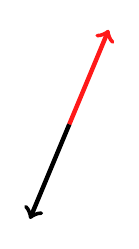
\begin{tikzpicture}
\draw [->, ultra thick, color=red!90] (0.0,0.0) -- (0.5,1.2);
\draw [->, ultra thick] (-0.0,-0.0) -- (-0.5,-1.2);
\end{tikzpicture}
& 
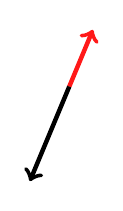
\begin{tikzpicture}
\draw [->, ultra thick, scale=0.6, color=red!90] (0.0,0.0) -- (0.5,1.2);
\draw [->, ultra thick] (-0.0,-0.0) -- (-0.5,-1.2);
\end{tikzpicture} 
&
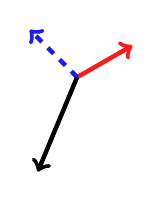
\begin{tikzpicture}
\draw [->, ultra thick, color=red!90] (0.0,0.0) -- (0.7,0.4);
\draw [->, ultra thick, dashed, color=blue!90] (0.0,0.0) -- (-0.6,0.6);
\draw [->, ultra thick] (-0.0,-0.0) -- (-0.5,-1.2);
\end{tikzpicture} 
 \\
$\alphat = \frac{1}{2}$ & $\alphat < \frac{1}{2}$ & $\alphat > \frac{1}{2}$
\end{tabular}
\end{center}
~\\
~\\
~\\
}
\frame{
\begin{figure}[h!t]
  \begin{center}
    \subfigure[\label{fig:alphat_le3j}$\njetlow$]{
      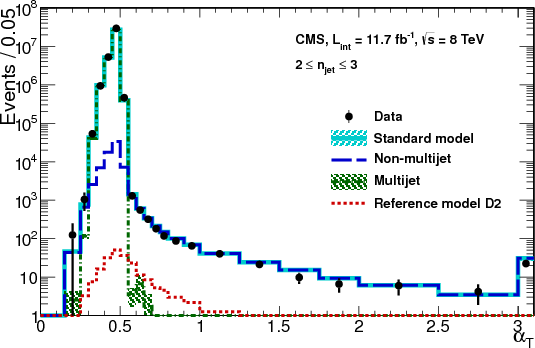
\includegraphics[width=0.60\textwidth,]{../figures/data-mc/AlphaT_le3j.png}
    } 
      \caption{\label{fig:alphat-2011} The $\alphat$ distribution for 11.7~fb$^{-1}$ 
            of data collected at {8}~\tev as well as for all SM
            backgrounds and one example SUSY signal sample, from Ref.~\cite{RA1Paper2012}.
            This figure is for illustrative purposes only, as this analysis relies
            on data control samples to estimate contribution from SM process 
            with genuine \met.}
    \label{fig:alphat_dist}
  \end{center}
\end{figure}

}

\frame{
\frametitle{HT $\times$ $\alphat$ Trigger}

innefficiency in trigger:
\begin{itemize}
\item Online: calo jets $\rightarrow$ Offline: PF jets
\end{itemize}

\begin{center}
\begin{table}[!h]
  \centering
  \scriptsize
  %\footnotesize
  \begin{tabular}{ ccccc }
    \hline
    \hline
    Offline \scalht       & Offline \alphat &  Trigger (HLT)  & \multicolumn{2}{c}{Efficiency (\%)}          \\ [0.5ex]
    bin (\gev)         & threshold       &                         & $2 \leq \njet \leq 3$ & $\njet \geq 4$       \\ [0.5ex]
    \hline
    $375 < \scalht < 475$ & 0.55          & HT300\_AlphaT0p53 & $94.2^{+0.5}_{-0.6}$  & $90.5^{+1.2}_{-1.3}$ \\
    $475 < \scalht < 575$ & 0.55          & HT350\_AlphaT0p52 & $96.2^{+0.8}_{-0.9}$  & $94.6^{+1.2}_{-1.4}$ \\
    $575 < \scalht < 675$ & 0.55          & HT400\_AlphaT0p51 & $95.4^{+1.4}_{-1.8}$  & $98.7^{+0.7}_{-1.12}$ \\
    $\scalht > 675$       & 0.55          & HT400\_AlphaT0p51 & $100^{+0.0}_{-2.0}$  & $100^{+0.0}_{-2.0}$ \\
    \hline
    \hline
  \end{tabular}
\end{table}

\end{center}

Muon control samples: IsoMu24\_eta2p1 88\%\\

Photon control sample: Photon150 100\% for $p_{T} > 165~\gev$

}

\frame{
\frametitle{HT $\times$ $\alphat$ Trigger}
\begin{figure}[!h]
  \footnotesize
  \begin{center}
    
\includegraphics[width=0.4\textwidth,page=30]{../figures/trigger/plotDump/v29/HT375_475_100_100_50_AlphaT_HT300xaT0p53_PF_le3j_RunAtFNAL.pdf}~~~~~~
    
\includegraphics[width=0.4\textwidth,page=30]{../figures/trigger/plotDump/v29/HT375_475_100_100_50_AlphaT_HT300xaT0p53_PF_ge4j_RunAtFNAL.pdf}\\
    \njetlow, $375 < \scalht < 475 \gev$~~~~
    \njethigh, $375 < \scalht < 475 \gev$\\
~\\
    
\includegraphics[width=0.4\textwidth,page=30]{../figures/trigger/plotDump/v29/HT475_575_100_100_50_AlphaT_HT350xaT0p52_PF_le3j_RunAtFNAL.pdf}~~~~~~
    
\includegraphics[width=0.4\textwidth,page=30]{../figures/trigger/plotDump/v29/HT475_575_100_100_50_AlphaT_HT350xaT0p52_PF_ge4j_RunAtFNAL.pdf}\\
    \njetlow, $475 < \scalht < 525 \gev$~~~~
    \njethigh, $475 < \scalht < 525 \gev$\\

  \end{center}
\end{figure}

}

\frame{
\frametitle{Event Selection}

Hadronic:
\begin{itemize}
\item $\scalht > 375~\gev$; jet 2 $p_{T} > 100~\gev$
\item No isolated $\mu$ or $e$ with $\pt > 10 \gev$
\item $\mht/\met < 1.25$
\item $\Delta$R(jet, dead ECAL region) $>$ 0.3 when $\Delta \phi^{*}$
\item HBHE Noise and $\met$ filters
\end{itemize}
~\\
Control: req's above +
\begin{itemize}
\item photon $\pt > 165~\gev, |\eta| < 1.4442$
\item one isolated muon $\pt > 25~\gev$
\item no $\alphat$ cut for muon samples\\
~~~$\Longrightarrow$ higher statistics\\
~~~$\Longrightarrow$ reduced S/B from signal contamination
\end{itemize}
}


\frame{
\frametitle{Example data-MC comparison plots 1}
\begin{figure}[h!]
  \centering
  \subfigure[\njet distribution ($\njet \geq 2$, $\nb \geq 0$).]{
    \label{fig:figures_JetMulti_all}
    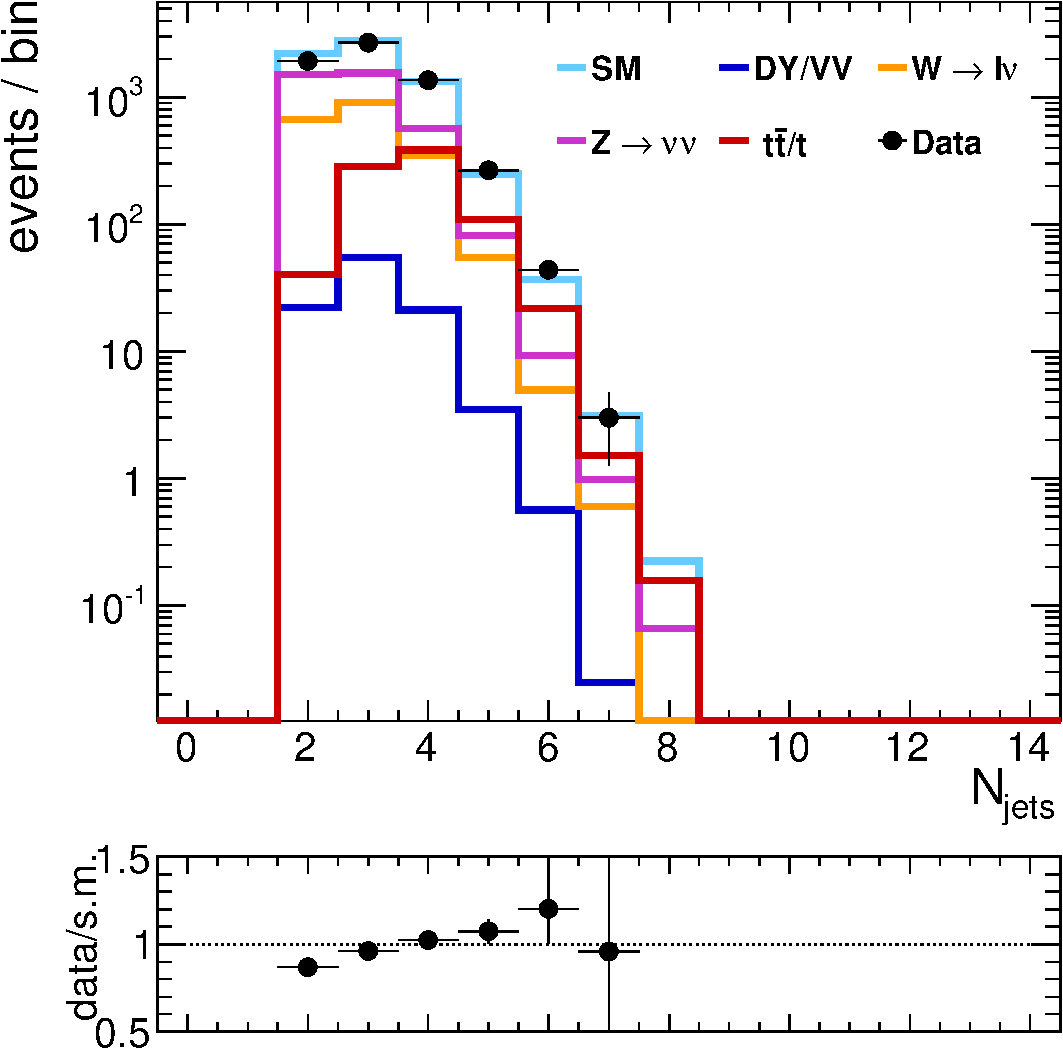
\includegraphics[width=0.4\paperwidth]{../figures/data-mc/v22/had/hadronicLook_375_pfJet_ge2j_xcak5JetPFIndicesPat.pdf}
  } 
  \subfigure[\nb distribution ($\njet \geq 2$, $\nb \geq 0$)]{
    \label{fig:figures_Bjet_all}
    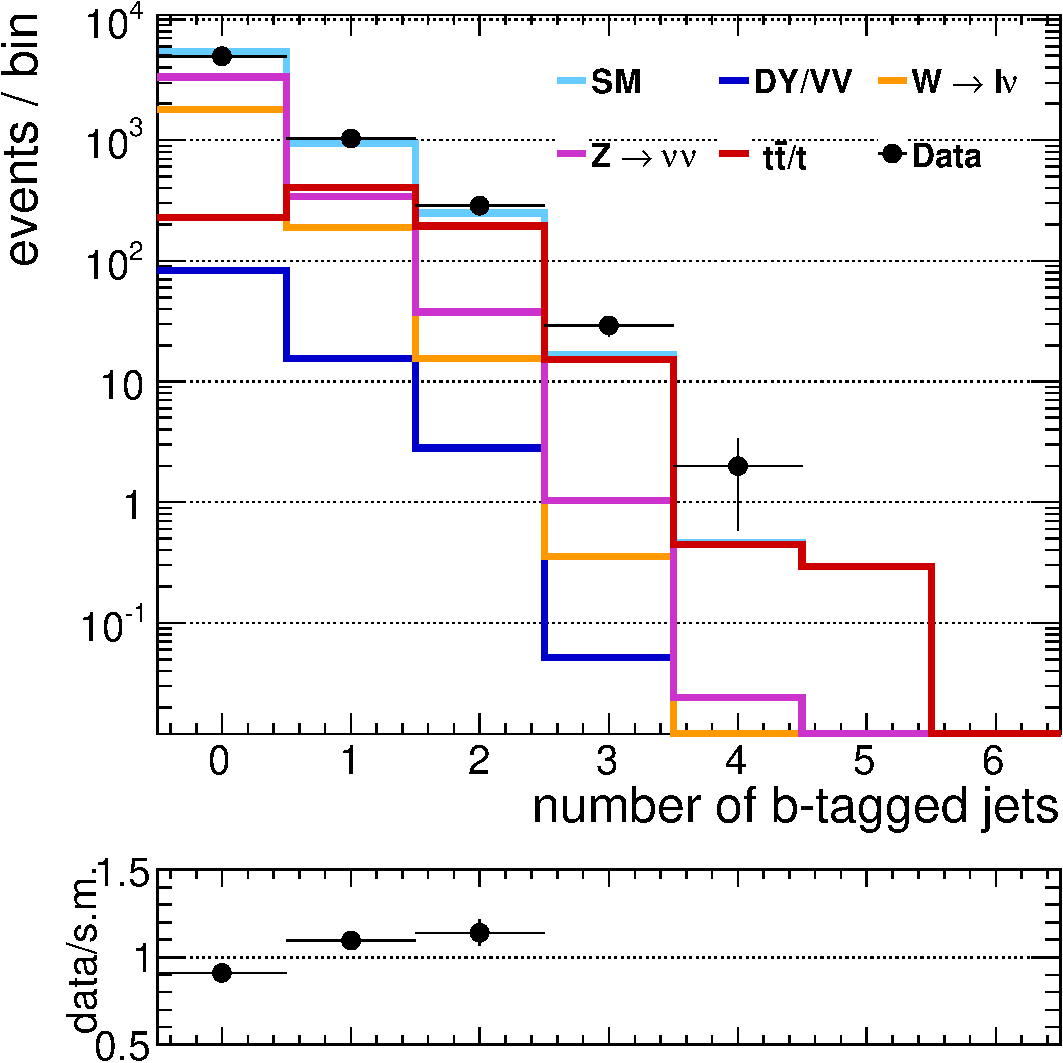
\includegraphics[width=0.4\paperwidth]{../figures/data-mc/v22/had/hadronicLook_375_pfJet_ge2j_xcak5JetPFIndicesBtagged2Pat.pdf}
  } \\
\end{figure}
}

\frame{
\frametitle{Example data-MC comparison plots 2}
\begin{figure}[h!]
  \centering
  \subfigure[\mht distribution ($\njet \geq 2$, $\nb \geq 0$)]{
    \label{fig:figures_MHT_0}
    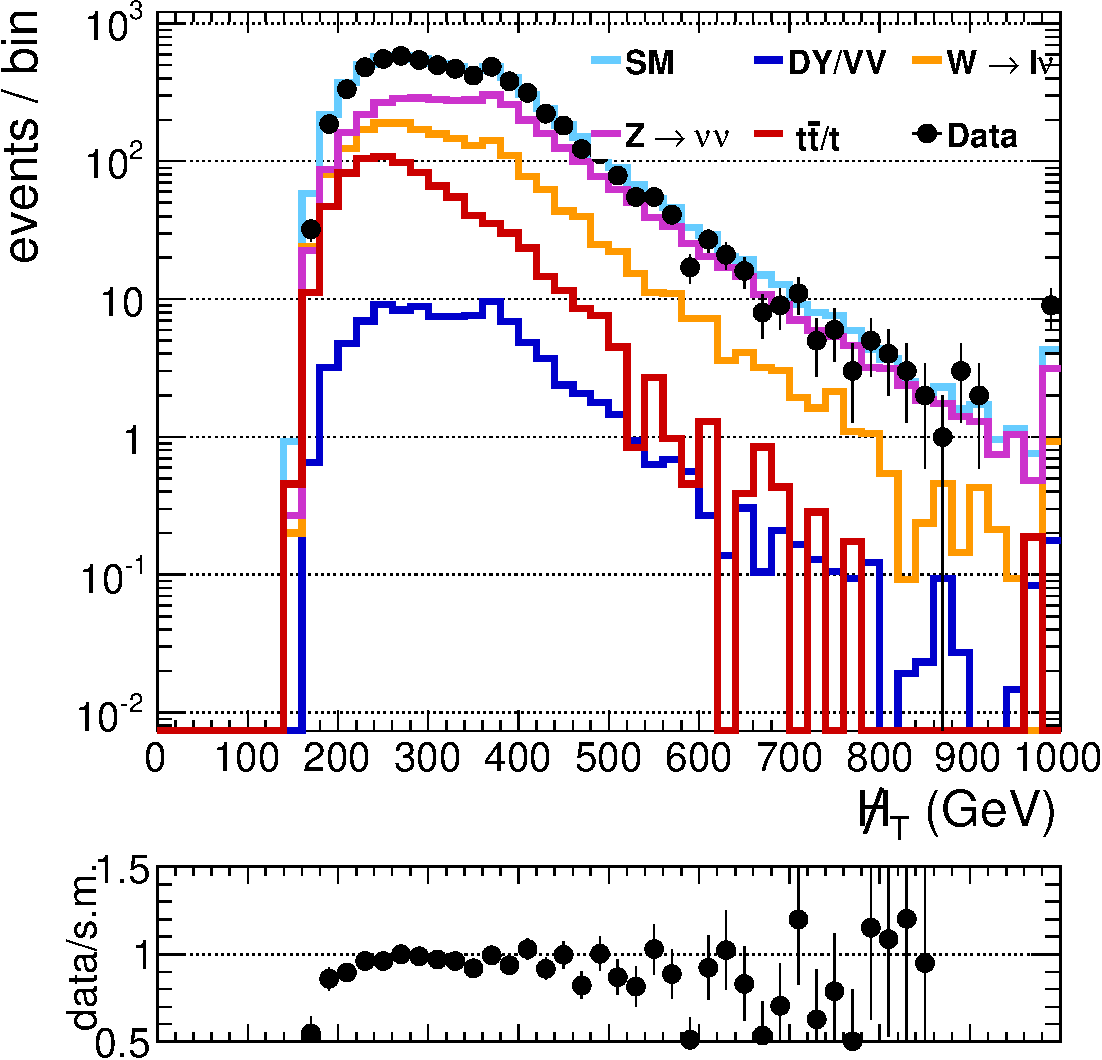
\includegraphics[width=0.4\paperwidth]{../figures/data-mc/v22/had/hadronicLook_375_pfJet_ge2j_xcak5JetPFMhtPat.pdf}
  } 
  \subfigure[\met distribution ($\njet \geq 2$, $\nb \geq 0$)]{
    \label{fig:figures_MET_1}
    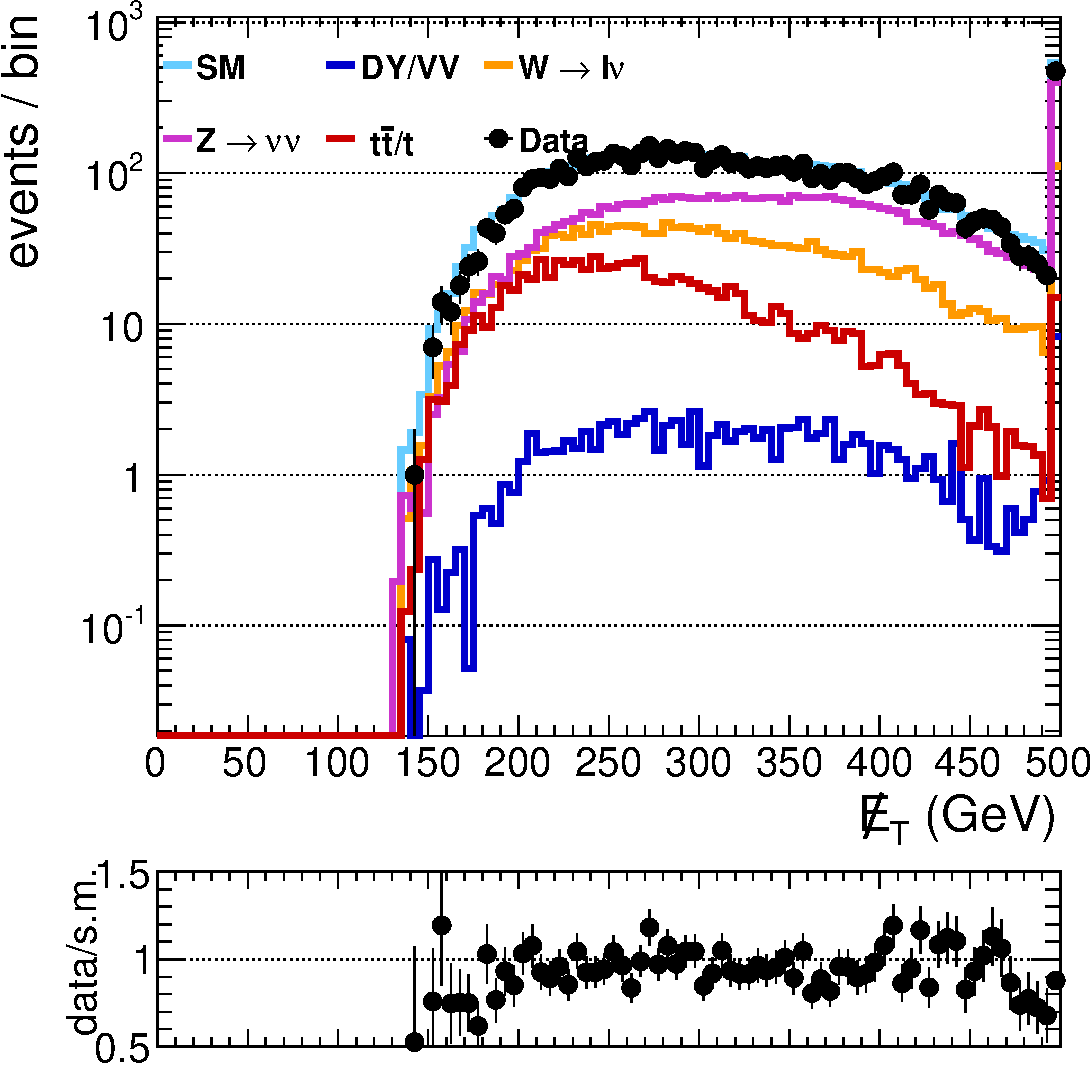
\includegraphics[width=0.4\paperwidth,]{../figures/data-mc/v22/had/hadronicLook_375_pfJet_ge2j_metP4TypeIPF.pdf}
  } \\
\end{figure}
}
\frame{
\frametitle{Example data-MC comparison plots 3}
\begin{figure}
  \centering
  \subfigure[\scalht distribution (\njetlow, $\nb = 0$)]{
    \label{fig:figures_HT_0}
    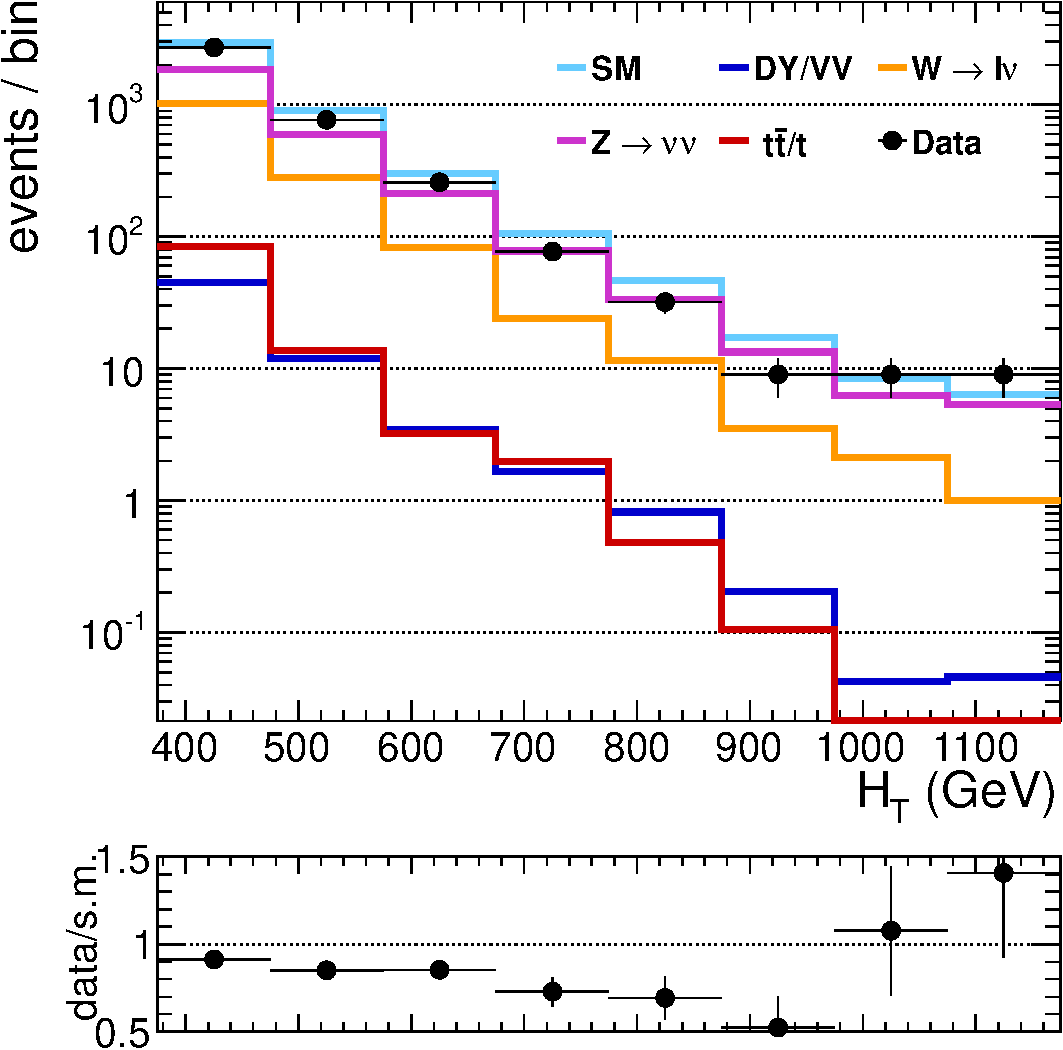
\includegraphics[width=0.4\paperwidth]{../figures/data-mc/v22/had/hadronicLook_375_pfJet_ge2j_xcak5JetPFSumEtPat_le3j_eq0b.pdf}
  } 
  \subfigure[\scalht distribution (\njethigh, $\nb = 1$)]{
    \label{fig:figures_HT_1}
    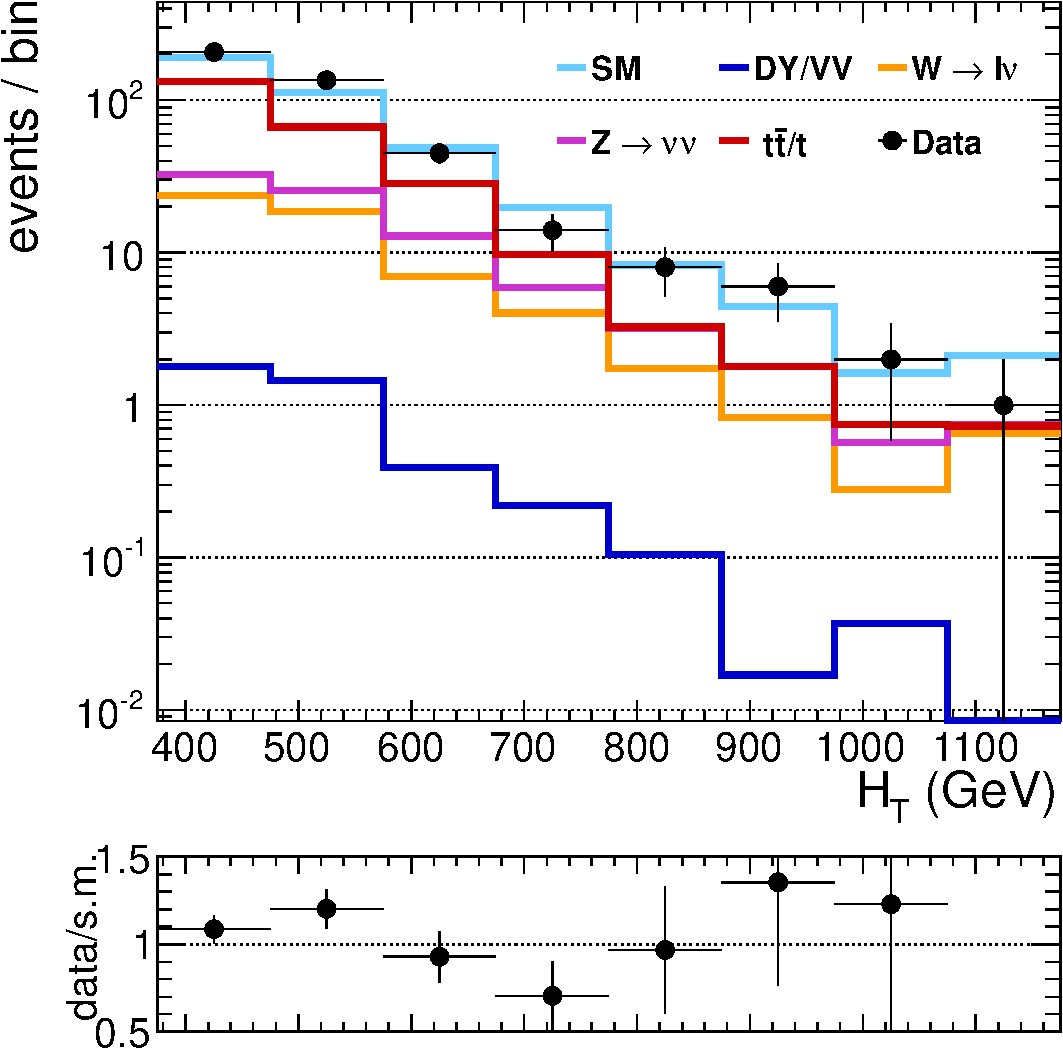
\includegraphics[width=0.4\paperwidth]{../figures/data-mc/v22/had/hadronicLook_375_pfJet_ge2j_xcak5JetPFSumEtPat_ge4j_eq1b.pdf}
  } \\
%\begin{figure}[h!]
%  \centering
%  \subfigure[\njet distribution ($\njet \geq 2$, $\nb \geq 0$).]{
%    \label{fig:figures_JetMulti_all}
%    \includegraphics[width=0.4\textwidth,page=89]{figures/data-mc/v22/had/hadronicLook_375_pfJet_ge2j.pdf}
%  } 
%  \subfigure[\nb distribution ($\njet \geq 2$, $\nb \geq 0$)]{
%    \label{fig:figures_Bjet_all}
%    \includegraphics[width=0.4\textwidth,page=100]{figures/data-mc/v22/had/hadronicLook_375_pfJet_ge2j.pdf}
%  } \\
%  \subfigure[\mht distribution ($\njet \geq 2$, $\nb \geq 0$)]{
%    \label{fig:figures_MHT_0}
%    \includegraphics[width=0.4\textwidth,page=83]{figures/data-mc/v22/had/hadronicLook_375_pfJet_ge2j.pdf}
%  } 
%  \subfigure[\mht distribution ($\njet \geq 2$, $\nb \geq 0$)]{
%    \label{fig:figures_MET_1}
%    \includegraphics[width=0.4\textwidth,page=69]{figures/data-mc/v22/had/hadronicLook_375_pfJet_ge2j.pdf}
%  } \\
%  \subfigure[\scalht distribution (\njetlow, $\nb = 0$)]{
%    \label{fig:figures_HT_0}
%    \includegraphics[width=0.4\textwidth,page=123]{figures/data-mc/v22/had/hadronicLook_375_pfJet_ge2j.pdf}
%  } 
%  \subfigure[\scalht distribution (\njethigh, $\nb = 1$)]{
%    \label{fig:figures_HT_1}
%    \includegraphics[width=0.4\textwidth,page=119]{figures/data-mc/v22/had/hadronicLook_375_pfJet_ge2j.pdf}
%  } \\
%  \caption{\label{fig:control-plots-sig} Data--MC comparisons of key
%    variables for the hadronic search region, following the
%    application of the full hadronic selection criteria and the
%    requirements $\scalht > 375\GeV$ and $\alphat > 0.55$: (a) \njet,
%    (b) \nb, (c) \mht, and (d) \met distributions for an inclusive 
%    selection on \njet and \nb, and (e,f) \scalht  for the two 
%    event categories (\njetlow, $\nb = 0$) and (\njethigh, $\nb = 1$). }
\end{figure}
}

\frame{
\frametitle{Translation Factors}

Translation factors = ratio of MC yields 

\begin{equation*}
  \label{equ:pred-method}
  \npre^{\rm had} = \underbrace{\frac{N_{\rm MC}^{\rm
      had}}{N_{\rm MC}^{\rm
      control}}}_\text{translation factor}\! \times \; \nobs^{\rm    control},   
\end{equation*}

Benefits:
\begin{itemize}
\item reduced dependence on accuracy of MC modelling
\item control and hadronic regions: 
  \begin{itemize}
  \item binned identically 
  \item kinematically similar, 
  \item similar admixtures of SM bkgds
  \end{itemize}
\item $N_{MC}^{had}$ and $N_{MC}^{control}$ are strongly correlated, biases largely cancel

\color{red!80}Checks for biases provided by, and systematics derived from, closure testsa
\end{itemize}
}

\frame{
\frametitle{Translation Factors}

\begin{itemize}
\item statistically independent
\item uncover biases
\item determine background 
\end{itemize}

Tests:
\begin{itemize}
\item $\alphat < 0.55 \rightarrow \alphat > 0.55$: check \mj 
\item between b-tag multiplicities: check bkg ad-mixture
\item between \njet multiplicities: check jes, kinetmatics 
\end{itemize}
~\\
\begin{equation*}
  \label{equ:tf-ratio-closure}
  \frac{N_{\rm MC}^{\rm \mj}(\scalht,\njethigh, \nb=1)}{N_{\rm MC}^{\rm \mj}(\scalht,\njetlow,\nb=1)} 
\end{equation*}
}

\frame{ 
\frametitle{Closure Tests}

\begin{figure}[h!]
  \begin{center}
    \subfigure[$2 \leq \njet \leq 3$\label{fig:closure_le3j}]{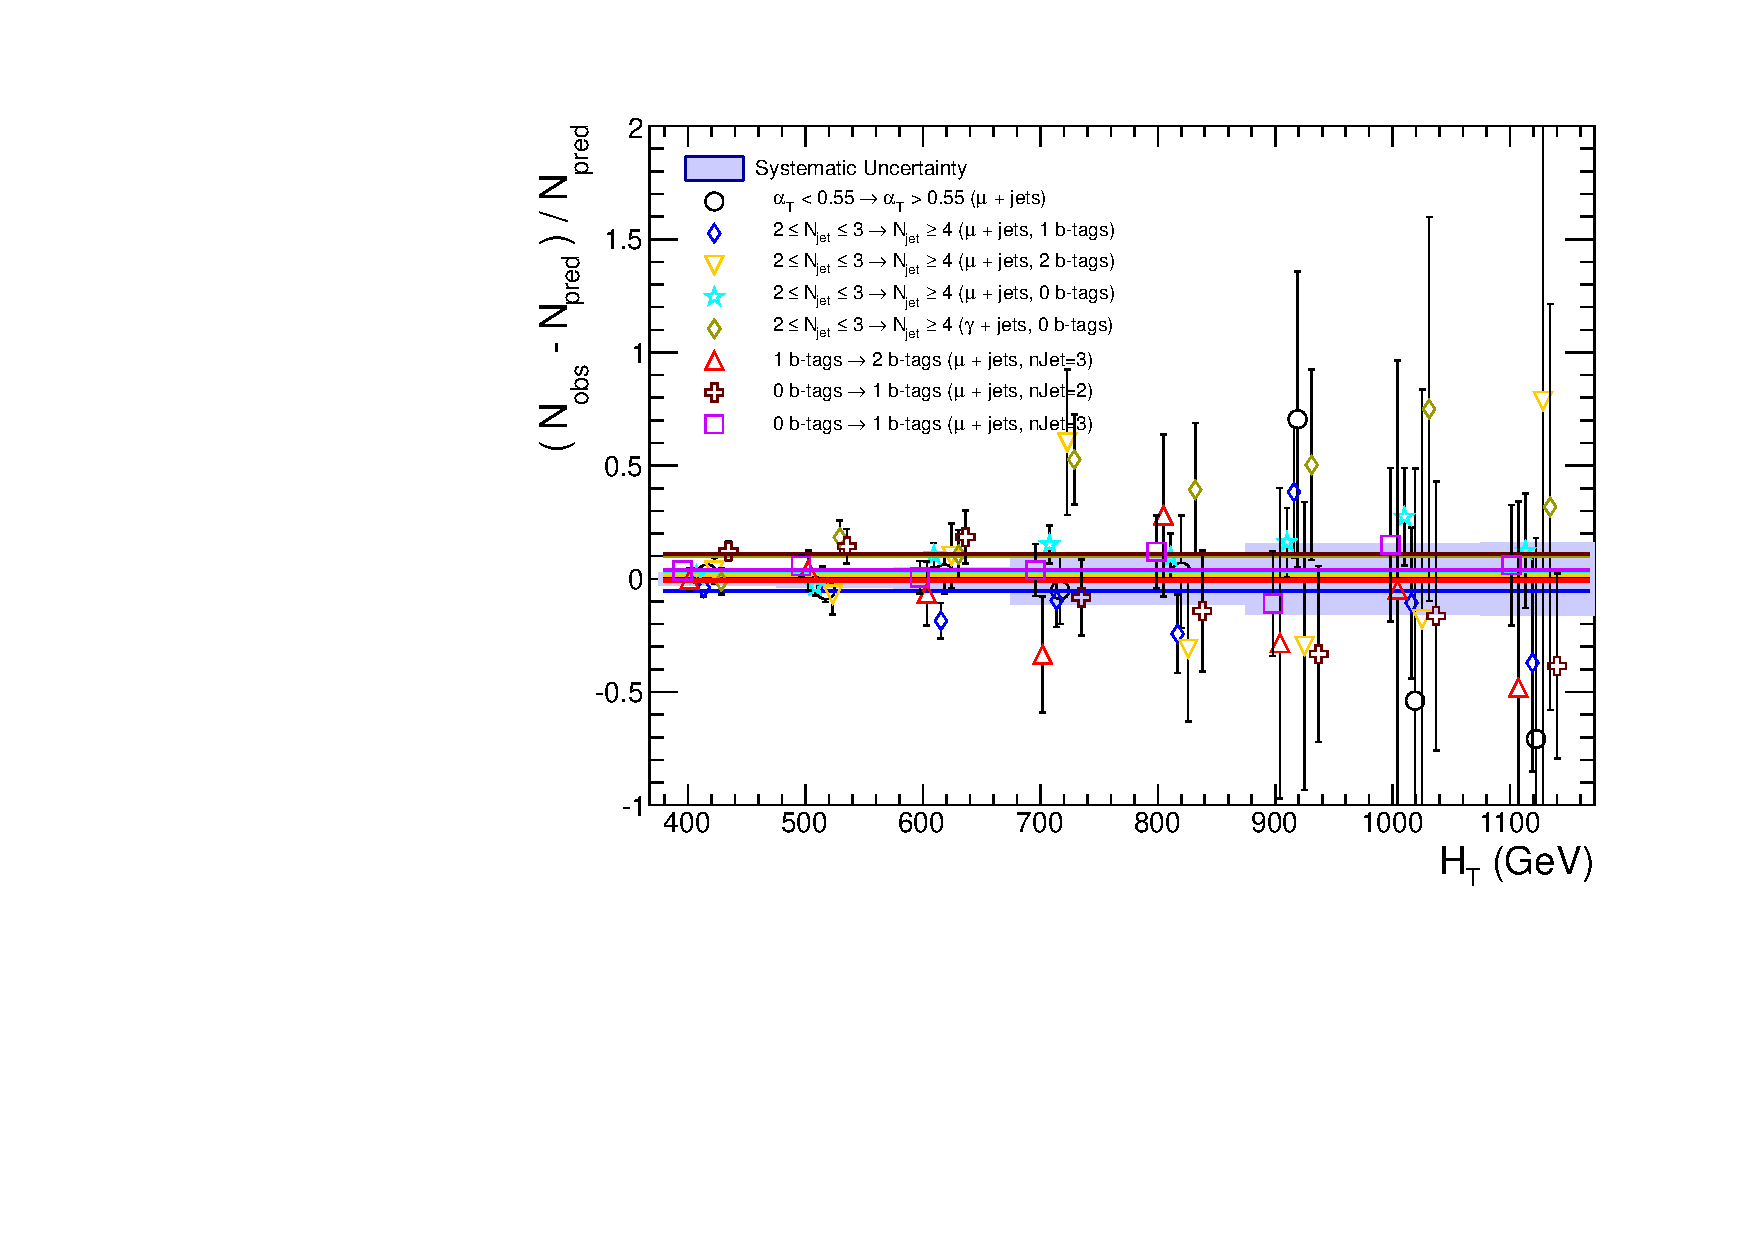
\includegraphics[width=0.8\textwidth]{../figures/syst/closureTests_pf_take21_le3j.pdf}}
     \label{fig:closure}
  \end{center} 
\end{figure}
}


\frame{ 
\frametitle{Closure Tests}

\begin{figure}[h!]
  \begin{center}
     \subfigure[$\njet \geq 4$]{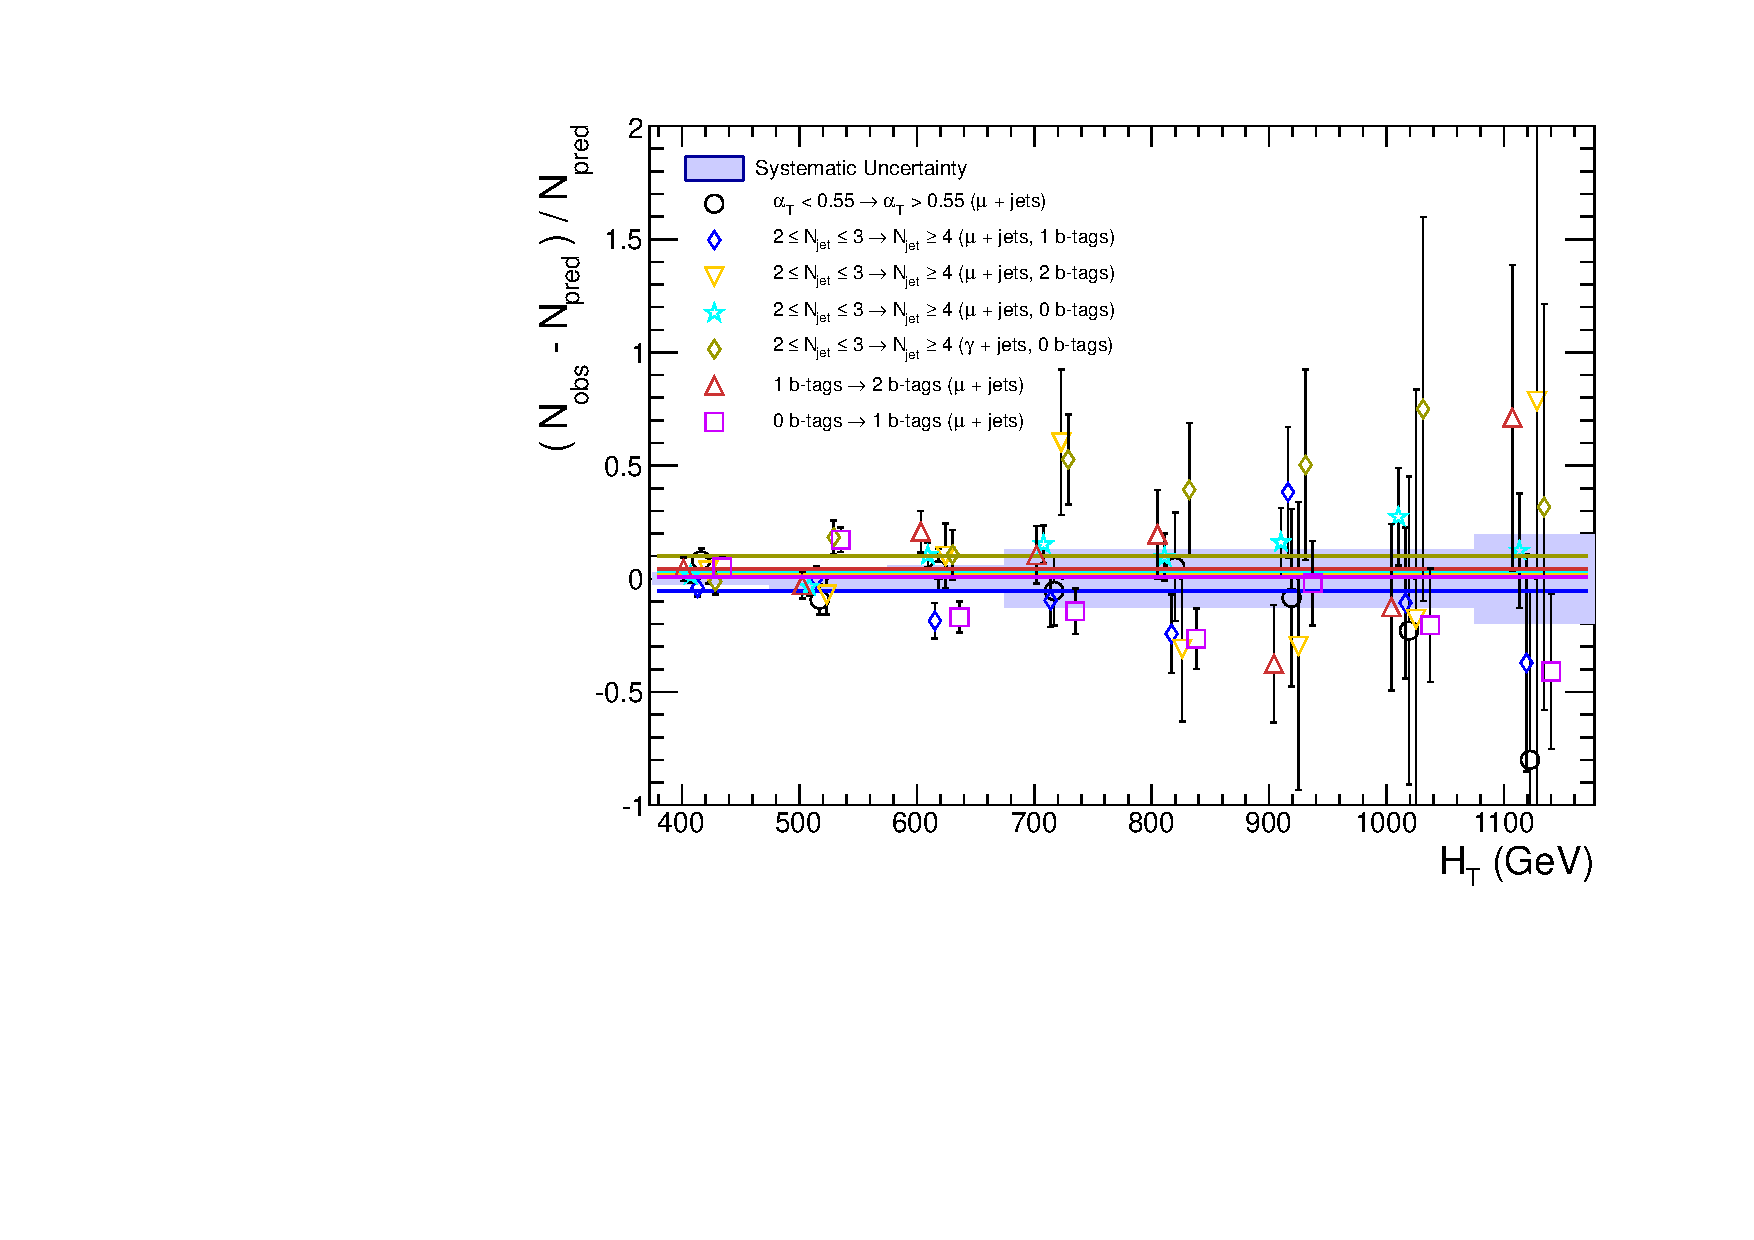
\includegraphics[width=0.8\textwidth]{../figures/syst/closureTests_pf_take21_ge4j.pdf}} \\
  \end{center} 
\end{figure}
}

\frame{
\frametitle{Background Uncertainty}

In addition:
\begin{itemize}
\item trigger: 5\%
\end{itemize}

%\begin{table}[!h]
%  \caption{A summary of the magnitude of the total systematic uncertainties (\%)
%    assigned to the translation factors, according to \njet and \scalht
%    bin.}
%  \label{tab:total-syst-values}
%  \centering
%  \tiny
%  \begin{tabular}{ ccccccccc }
%    \hline
%    \hline
%            & \multicolumn{7}{c}{\scalht bin (GeV)}                                \\
%    \cline{2-9}
%    \njet   & 375--475 & 475--525 & 525--675 & 675--775 & 775--875 & 875-975 & 975-1075 & $>1075$ \\
%    \hline                                                                                                                                  
%    2--3    & 6        & 6        & 7        & 12       & 12       & 17      & 17        & 17     \\
%    $\geq$4 & 6        & 6        & 8        & 14       & 14       & 14      & 14        & 21     \\
%    \hline                                                                                                                                  
%    \hline
%  \end{tabular}
%\end{table}

\begin{table}[!h]
  \caption{A summary of the magnitude of the total systematic uncertainties (\%)
    assigned to the translation factors, according to \njet and \scalht
    bin.}
  \label{tab:total-syst-values}
  \centering
  \scriptsize
  \begin{tabular}{ ccccccccc }
    \hline
    \hline
            & \multicolumn{7}{c}{\scalht bin (GeV)}                                \\
    \cline{2-9}
\\
    \njet   & 375 & 475 & 525 & 675 & 775 & 875 & 975 & $>1075$ \\
    \hline                                                                                                                                  
    2--3    & 6        & 6        & 7        & 12       & 12       & 17      & 17        & 17     \\
    $\geq$4 & 6        & 6        & 8        & 14       & 14       & 14      & 14        & 21     \\
    \hline                                                                                                                                  
    \hline
  \end{tabular}
\end{table}

}

\section{Results}
\subsection{Likelihood}{
\frame{
\frametitle{Likelihood Model Overview}

Setup:

\begin{itemize}
\item Each observation is modeled as Poisson
\item Hadronic SM EWK expectations are related to $\mu$, $\gamma$
expectations via ``translation factors'' from MC
\end{itemize}

Pick a signal model, a given value of signal cross section
(e.g. 0=SM or 1=nominal), and a particular category of \nb. The
parameters floated are:
\begin{itemize}
\item the yields of SM EWK events in each hadronic bin
\item those determining the relative contributions from ($t$ $\rightarrow$) W
and Z
\item those accommodating systematic uncertainty on the
  background translations and on the signal efficiency
\end{itemize}
}

\frame{
\setlength{\belowdisplayskip}{0pt} \setlength{\belowdisplayshortskip}{1pt}
\setlength{\abovedisplayskip}{0pt} \setlength{\abovedisplayshortskip}{1pt}
\frametitle{The Likelihood}
\begin{equation*}
L^k = L_{hadronic}^k \times L_{\mu}^k \times L_{\gamma}^k \times
L_{\rm EWK\, syst.}^k \quad
\end{equation*}
~\\
\visible<2,3,4>{For a given an analysis category,}
\visible<2,3,4>{\begin{equation*}
L_{hadronic}=\prod_i \mathrm{Pois}(n^i |\, b^i + s^i)
\label{eq:hadronicLikelihood}
\end{equation*}
for \scalht bin $i$. }
\visible<3,4>{\begin{equation*}
\label{eq:photonLikelihood}
L_{\gamma}= \prod_i \mathrm{Pois}(n_{\gamma}^i |\, \rho_{\gamma Z}^i \cdot
r_{\gamma}^{i} \cdot \zInv{i})
\end{equation*}}

\visible<3,4>{\begin{equation*}
\label{eq:muonLikelihood}
L_{\mu}=\prod_i \mathrm{Pois}(n_{\mu}^i |\, \rho_{\mu W}^i \cdot
r_{\mu}^{i} \cdot ttW^{i})\quad
\end{equation*}}

\visible<4>{\begin{equation*}
r_{\gamma}^i = \frac{MC_{\gamma}^i}{MC_{\zInv{}}^i};\, r_{\mu}^i =
\frac{MC_{\mu}^i}{MC_{t\bar{t}+W}^i}\quad
\end{equation*}}
}

%\visible<3,4>{\begin{equation*}
%\label{eq:muonLikelihood}
%L_{\mu}=\prod_i \mathrm{Pois}(n_{\mu}^i |\, \rho_{\mu W}^i \cdot
%r_{\mu}^{i} \cdot ttW^{i})\quad
%\end{equation*}}
%
%\visible<4>{\begin{equation*}
%r_{\gamma}^i = \frac{MC_{\gamma}^i}{MC_{\zInv{}}^i};\, r_{\mu}^i =
%\frac{MC_{\mu}^i}{MC_{t\bar{t}+W}^i}\quad ,
%\end{equation*}}


\frame{
\setlength{\belowdisplayskip}{3pt} \setlength{\belowdisplayshortskip}{1pt}
\setlength{\abovedisplayskip}{3pt} \setlength{\abovedisplayshortskip}{1pt}
\frametitle{The Likelihood}
\begin{equation*}
L^k = L_{hadronic}^k \times L_{\mu}^k \times L_{\gamma}^k \times
L_{\rm EWK\, syst.}^k \quad
\end{equation*}

\begin{equation*}
\label{eq:ewkSyst}
L_{\rm EWK\, syst.}=\prod_i \mathrm{Logn}( 1.0 |\,\rho_{\mu W}^i,
\sigma_{\mu W}^i)\times \mathrm{Logn}( 1.0 |\,\rho_{\gamma Z}^i,
\sigma_{\gamma Z}^i) \quad
\end{equation*}

where Logn is the log-normal
distribution~\cite{cousins-log-normal}:

\begin{equation*}
\label{eq:log-normal}
\mathrm{Logn}(x |\,\mu,\sigma_{\mathrm{rel.}}) =
\frac{1}{x\sqrt{2\pi}\ln{k}}\exp{\left(-\frac{\ln^2{\left(\frac{x}{\mu}\right)}}{2\ln^2{k}}\right)};\quad
k=1+\sigma_{\mathrm rel.}\quad. 
\end{equation*}
\begin{itemize}
\item non-negative
\item relative uncertainty 
\end{itemize}
}


\frame{
\frametitle{$\njetlow$, 0b}
\begin{figure}[t!]
  \begin{center}
    %\stackunder[5pt]{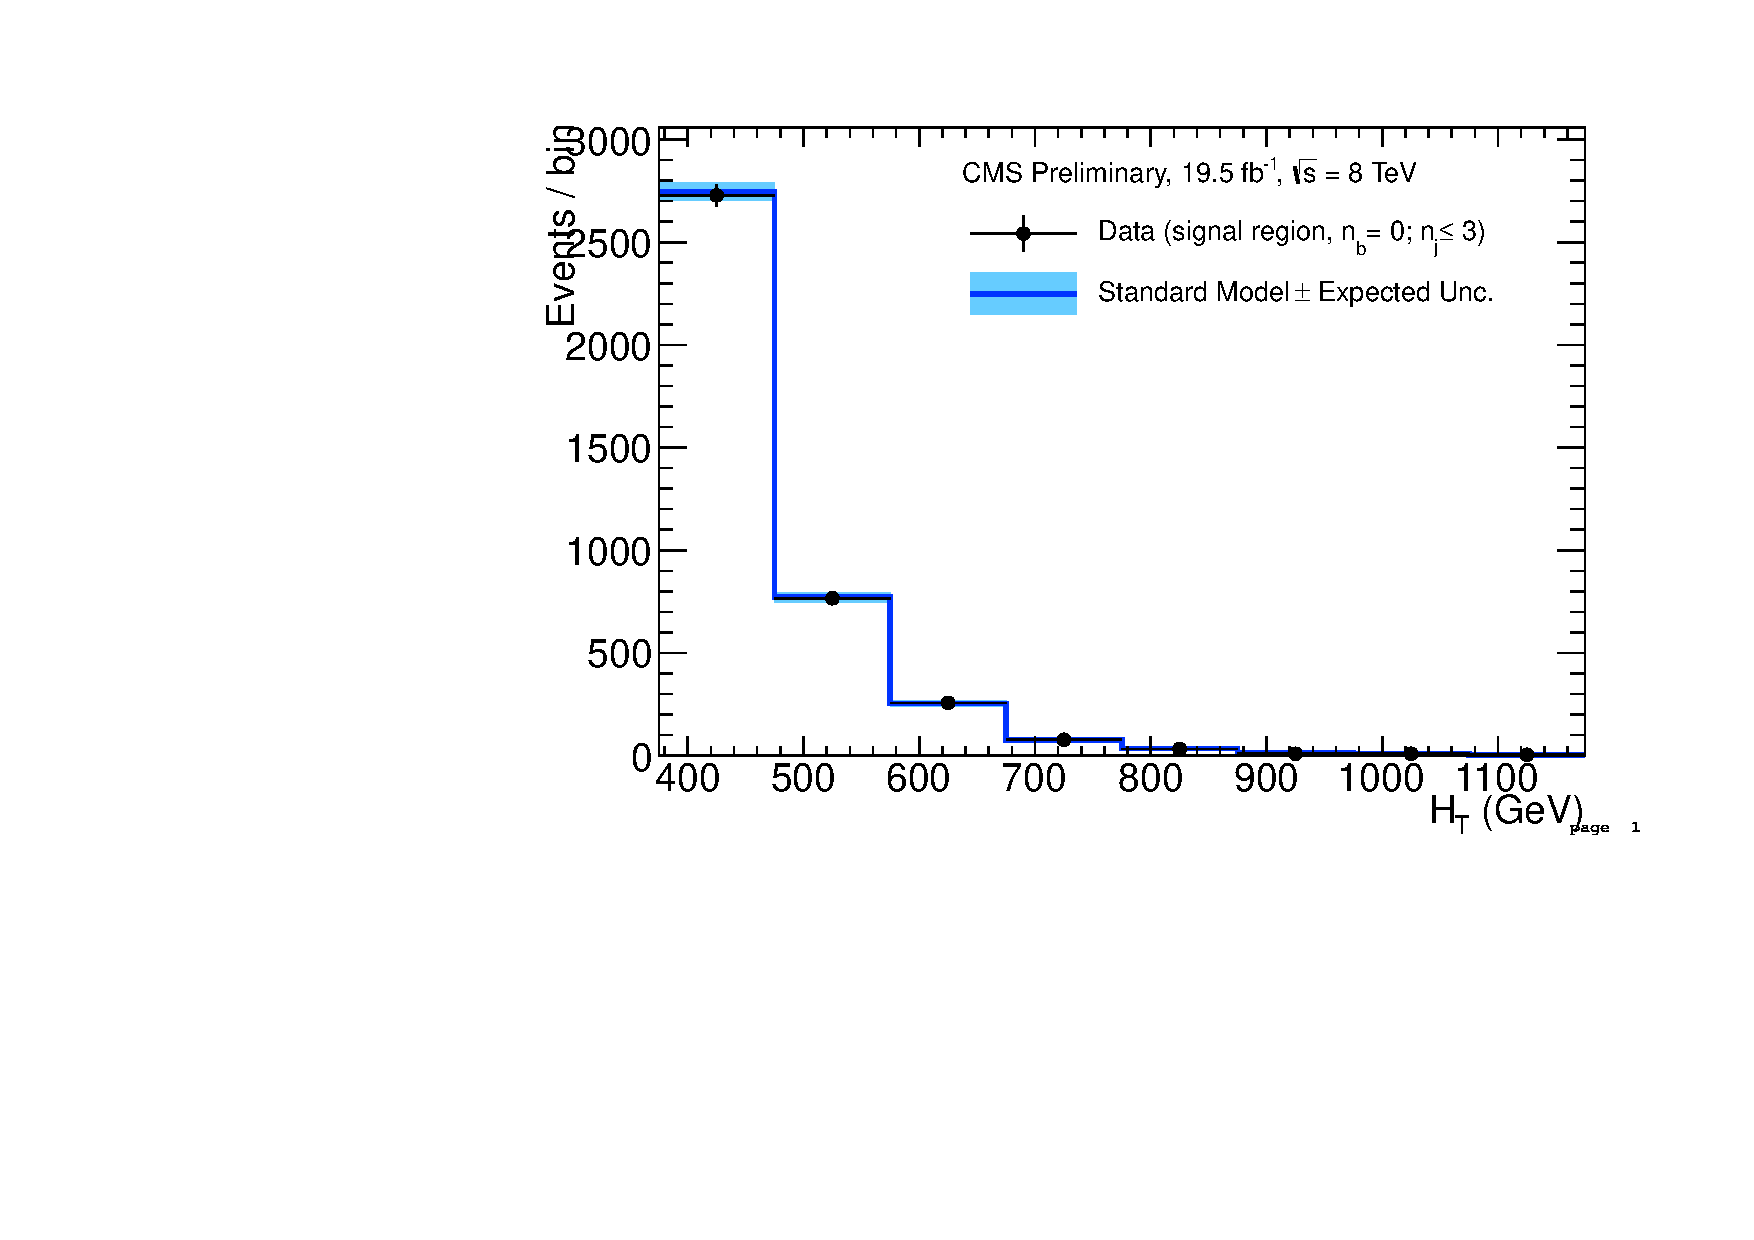
\includegraphics[width=2in,height=.7in]{../figures/fit/v22/bestFit_2012pf_RQcdZero_fZinvAll_0b_le3j-1hp_smOnly}}{Hadronic sample (lin. scale)}%
    \subfigure[Hadronic sample (lin. scale)]{
      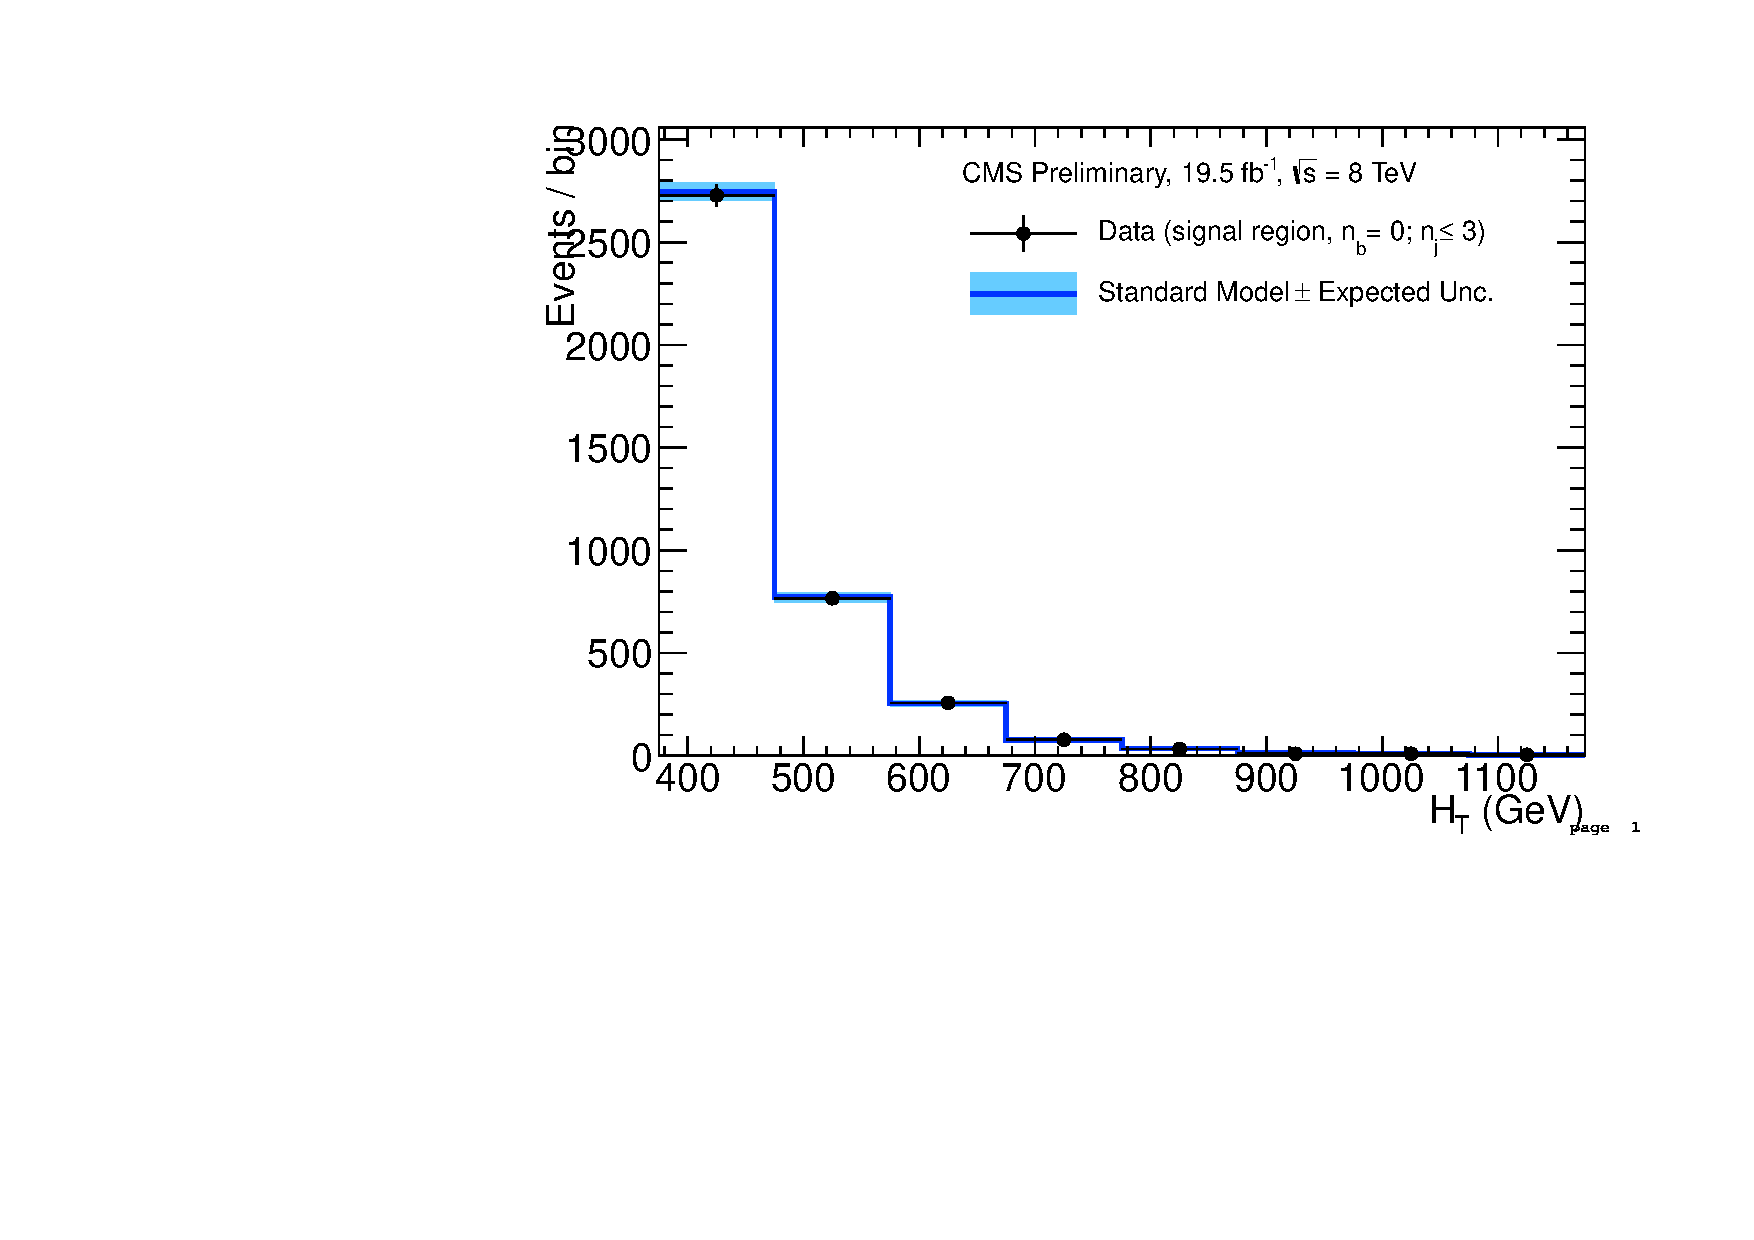
\includegraphics[width=0.40\textwidth,page=1]{../figures/fit/v22/bestFit_2012pf_RQcdZero_fZinvAll_0b_le3j-1hp_smOnly}
    } 
    \subfigure[Hadronic sample (log. scale)]{
      \includegraphics[width=0.40\textwidth,page=2]{../figures/fit/v22/bestFit_2012pf_RQcdZero_fZinvAll_0b_le3j-1hp_smOnly}
    } \\
    \subfigure[$\mu$ + jets sample]{
      \includegraphics[width=0.40\textwidth,page=4]{../figures/fit/v22/bestFit_2012pf_RQcdZero_fZinvAll_0b_le3j-1hp_smOnly}
    } 
    \subfigure[$\gamma$ + jets sample]{
      \includegraphics[width=0.40\textwidth,page=6]{../figures/fit/v22/bestFit_2012pf_RQcdZero_fZinvAll_0b_le3j-1hp_smOnly}
    } 
  \end{center}
\end{figure}

}
}
\frame{
\frametitle{$\njethigh$, 0b}
\begin{figure}[t!]
  \begin{center}
    %\stackunder[5pt]{\includegraphics[width=2in,height=.7in]{../figures/fit/v22/bestFit_2012pf_RQcdZero_fZinvAll_0b_le3j-1hp_smOnly}}{Hadronic sample (lin. scale)}%
    \subfigure[Hadronic sample (lin. scale)]{
      \includegraphics[width=0.40\textwidth,page=1]{../figures/fit/v22/bestFit_2012pf_RQcdZero_fZinvAll_0b_ge4j-1hp_smOnly}
    } 
    \subfigure[Hadronic sample (log. scale)]{
      \includegraphics[width=0.40\textwidth,page=2]{../figures/fit/v22/bestFit_2012pf_RQcdZero_fZinvAll_0b_ge4j-1hp_smOnly}
    } \\
    \subfigure[$\mu$ + jets sample]{
      \includegraphics[width=0.40\textwidth,page=4]{../figures/fit/v22/bestFit_2012pf_RQcdZero_fZinvAll_0b_ge4j-1hp_smOnly}
    } 
    \subfigure[$\gamma$ + jets sample]{
      \includegraphics[width=0.40\textwidth,page=6]{../figures/fit/v22/bestFit_2012pf_RQcdZero_fZinvAll_0b_ge4j-1hp_smOnly}
    } 
  \end{center}
\end{figure}

}

\frame{
\frametitle{$\njethigh$, 1b}
\begin{figure}[t!]
  \begin{center}
    %\stackunder[5pt]{\includegraphics[width=2in,height=.7in]{../figures/fit/v22/bestFit_2012pf_RQcdZero_fZinvAll_0b_le3j-1hp_smOnly}}{Hadronic sample (lin. scale)}%
    \subfigure[Hadronic sample (lin. scale)]{
      \includegraphics[width=0.40\textwidth,page=1]{../figures/fit/v22/bestFit_2012pf_RQcdZero_fZinvAll_1b_ge4j-1hp_smOnly}
    } 
    \subfigure[Hadronic sample (log. scale)]{
      \includegraphics[width=0.40\textwidth,page=2]{../figures/fit/v22/bestFit_2012pf_RQcdZero_fZinvAll_1b_ge4j-1hp_smOnly}
    } \\
    \subfigure[$\mu$ + jets sample]{
      \includegraphics[width=0.40\textwidth,page=4]{../figures/fit/v22/bestFit_2012pf_RQcdZero_fZinvAll_1b_ge4j-1hp_smOnly}
    } 
    \subfigure[$\gamma$ + jets sample]{
      \includegraphics[width=0.40\textwidth,page=6]{../figures/fit/v22/bestFit_2012pf_RQcdZero_fZinvAll_1b_ge4j-1hp_smOnly}
    } 
  \end{center}
\end{figure}

}

\frame{
\frametitle{$\njetlow$, 2b}
\begin{figure}[t!]
    \subfigure[Hadronic sample (lin. scale)]{
      \includegraphics[width=0.40\textwidth,page=1]{../figures/fit/v22/bestFit_2012pf_RQcdZero_fZinvAll_2b_le3j-1h_smOnly}
    } 
    \subfigure[Hadronic sample (log. scale)]{
      \includegraphics[width=0.40\textwidth,page=2]{../figures/fit/v22/bestFit_2012pf_RQcdZero_fZinvAll_2b_le3j-1h_smOnly}
    } \\
    \subfigure[$\mu$ + jets sample]{
      \includegraphics[width=0.40\textwidth,page=4]{../figures/fit/v22/bestFit_2012pf_RQcdZero_fZinvAll_2b_le3j-1h_smOnly}
    } 
\end{figure}

}

\frame{
\frametitle{$\njethigh$, 2b}
\begin{figure}[t!]
    \subfigure[Hadronic sample (lin. scale)]{
      \includegraphics[width=0.40\textwidth,page=1]{../figures/fit/v22/bestFit_2012pf_RQcdZero_fZinvAll_2b_ge4j-1h_smOnly}
    } 
    \subfigure[Hadronic sample (log. scale)]{
      \includegraphics[width=0.40\textwidth,page=2]{../figures/fit/v22/bestFit_2012pf_RQcdZero_fZinvAll_2b_ge4j-1h_smOnly}
    } \\
    \subfigure[$\mu$ + jets sample]{
      \includegraphics[width=0.40\textwidth,page=4]{../figures/fit/v22/bestFit_2012pf_RQcdZero_fZinvAll_2b_ge4j-1h_smOnly}
    } 
\end{figure}
}

\frame{
\frametitle{p-values and pulls}
\begin{figure}[h!]
  \begin{center}
    \subfigure[p-values per event category.]{
      \includegraphics[width=0.4\paperwidth, trim=0 190 290 20, clip=true]{../figures/fit/v22/pValues} % lbrt
    } 
    \subfigure[Pull versus signal region bin.\label{fig:sigVsCat}]{
      \includegraphics[width=0.4\paperwidth, trim=0 0 0 30, clip=true]{../figures/fit/v22/significances_catVsHt_4}
    } \\
%    \subfigure[Pull per signal region bin.]{
%      \includegraphics[width=0.45\textwidth, trim=0 0 0 0, clip=true]{figures/fit/v1/pull_per_bin_gaus}
%    } 
%    \subfigure[p-value per signal region bin.]{
%      \includegraphics[width=0.45\textwidth, trim=0 0 0 0, clip=true]{figures/fit/v1/pvalue_per_bin}
%    } \\
    %\caption{Pulls and p-values. See text for details}
    \label{fig:fluct}
  \end{center}
\end{figure}
}

\frame{
\frametitle{Including the Signal Models}

\begin{equation*}
L = L_{sig.\,syst}^k \times \prod_k L_{hadronic}^k
\times L_{\mu}^k \times L_{ph}^k \times L_{\rm EWK\, syst.}^k \quad .
\end{equation*}

\begin{equation*}
L_{hadronic}=\prod_i \mathrm{Pois}(n^i |\, b^i + s^i)
\end{equation*}


\begin{center}
$s^i \equiv
f\rho_{sig} xl\epsilon_{had}^i$
\end{center}

\begin{equation*}
L_{sig.\,syst}=\mathrm{Logn}(1.0 |\,\rho_{sig}, \delta) \quad .
\end{equation*}
}
\subsection{Signal Model}
\frame{
\frametitle{example signal efficiencies}
\begin{figure}[h!]
  \begin{center}
%    \subfigure[Hadronic Selection Efficiency, (2--3,0)]{
%      \includegraphics[width=0.4\textwidth,page=6]{figures/sms/t2cc/v1/T2cc_eff}
%    } 
    \subfigure[T2cc, Hadronic Selection Efficiency, (2--3,1)]{
      \includegraphics[width=0.45\textwidth,page=7]{../figures/sms/t2cc/v1/T2cc_eff}
    } 
%    \subfigure[Hadronic Selection Efficiency, ($\geq 4$,0)]{
%      \includegraphics[width=0.4\textwidth,page=1]{figures/sms/t2cc/v1/T2cc_eff}
%    } 
%    \subfigure[Hadronic Selection Efficiency, ($\geq 4$,1)]{
%      \includegraphics[width=0.4\textwidth,page=2]{figures/sms/t2cc/v1/T2cc_eff}
%    } 
%    \caption{Hadronic selection efficiency times acceptance for \texttt{T2cc}
%      for the relevant event categories defined by \njet and \nb in the $m_{\st}$--$m_{LSP}$ plane.
%      Note the different z-axis scales.}
%    \label{fig:sms-eff-t2cc}
%  \end{center}
%\end{figure}
%
%\begin{figure}[!h]
%  \begin{center}
%    \subfigure[T2tt, Hadronic Selection Efficiency, ($\geq 4$,1)]{
%      \includegraphics[width=0.4\textwidth,page=2]{figures/sms/t2tt/v1/T2tt_eff}
%    } 
    \subfigure[Hadronic Selection Efficiency, ($\geq 4$,2)]{
      \includegraphics[width=0.45\textwidth,page=3]{../figures/sms/t2tt/v1/T2tt_eff}
    } \\
%    \caption{Hadronic selection efficiency times acceptance for the \texttt{T2tt}
%      for the relevant event categories defined by \njet and \nb in the $m_{\st}$--$m_{LSP}$ plane.
%       Note the different z-axis scales.}
%    \label{fig:sms-eff-t2tt}
  \end{center}
\end{figure}

}
\frame{
\frametitle{Uncertainty on Signal Efficiency}
\begin{itemize}
\item PDF - Parton Distribution Function
\item JES - Jet Energy Scale
\item ISR - Initial State Radiation
\end{itemize}
~\\
\begin{center}
T2cc
\end{center}
\begin{table}[h!]
%  \caption{Representative ranges for each contribution to the total
%    relative systematic uncertainty in the signal efficiency times acceptance
%    for each relevant event category for the \texttt{T2cc}
%    interpretation. The luminosity, trigger, and Dead Ecal uncertainties
%    are category indepedent i.e. they affect all categories equally. 
%    \label{tab:sms-syst-t2cc}
%  }   
  \centering
  \scriptsize
  \begin{tabular}{ lcccccc }
    \hline
    \hline
    Category   & \multicolumn{2}{c}{(2--3,0)} & \multicolumn{2}{c}{($\geq 4$,0)} & \multicolumn{2}{c}{($\geq 4$,1)}\\% & \multicolumn{2}{c}{($\geq 2$,$\geq 0$)} \\
    Range      & Min.   & Max.                & Min.   & Max.                    & Min. & Max.                    \\ % & Min.  & Max.        \\
    \hline                                                                                                         %
    PDF        & 0.00   & 0.05                & 0.00   & 0.05                    & 0.00 & 0.10                    \\ % &         \\
    JES        & 0.00   & 0.10                & 0.00   & 0.10                    & 0.00 & 0.15 	                  \\ % &             \\
    ISR        & 0.15   & 0.25                & 0.10   & 0.15                    & 0.15 & 0.30 	                  \\ % &             \\
    b-tag SF   & 0.00   & 0.08                & 0.00   & 0.10                    & 0.00 & 0.15 	                  \\ % &             \\
    \hline                                                                                                         %
    Luminosity & \multicolumn{6}{c}{0.026}                                                                      \\ %
    Trigger & \multicolumn{6}{c}{0.05}                                                                       \\ %
    Dead Ecal & \multicolumn{6}{c}{0.03}                                                                       \\ %
    %    Luminosity &         &                     &        &                         &      &      	          \\ %         & 0.026 & 0.026        \\
    %Trigger    &        &                     &        &                         &      &                        \\ %  & 0.05 & 0.05        \\
    %Dead Ecal  &        &                     &        &                         &      &      	          \\ %         & 0.03 & 0.03        \\
    \hline                                                                                                         %
    Total syst & 0.18   & 0.25                & 0.19   & 0.30                    & 0.20 & 0.38                    \\ % &      &             \\
    \hline
    \hline
  \end{tabular}
\end{table}
}
\frame{
\frametitle{Uncertainty on Signal Efficiency}
\begin{itemize}
\item PDF - Parton Distribution Function
\item JES - Jet Energy Scale
\item ISR - Initial State Radiation
\end{itemize}
~\\
\begin{center}
T2tt
\end{center}

\begin{table}[h!]
%  \caption{Representative ranges for each contribution to the total
%    systematic uncertainty in the signal efficiency times acceptance
%    for each relevant event category for the \texttt{T2tt}
%    interpretation. The luminosity, trigger, and Dead Ecal uncertainties
%    are category indepedent i.e. they affect all categories equally. 
%    \label{tab:sms-syst-t2cc}
%  }   
  \centering
  \scriptsize
  \begin{tabular}{ lcccccc }
    \hline
    \hline
    Category   & \multicolumn{2}{c}{($\geq 4$,1)} & \multicolumn{2}{c}{($\geq 4$,2)}\\%  & \multicolumn{2}{c}{($\geq 2$,$\geq 0$)} \\
    Range      & Min.   & Max.                & Min.   & Max.                     \\%& Min.  & Max.        \\
    \hline                                                                        %
    PDF        & 0.00   & 0.10                & 0.00   & 0.10                     \\%&         \\
    JES        & 0.00   & 0.10                & 0.00   & 0.05                     \\%&             \\
    ISR        & 0.00   & 0.20                & 0.00   & 0.22                     \\%&             \\
    b-tag SF   & 0.00   & 0.05                & 0.00   & 0.10                     \\%&             \\
    \hline                                                                        %
    Luminosity & \multicolumn{4}{c}{0.026}                                                                      \\ %
    Trigger & \multicolumn{4}{c}{0.05}                                                                       \\ %
    Dead Ecal & \multicolumn{4}{c}{0.03}                                                                       \\ %
    \hline                                                                                                         %    
    Total syst & 0.05   & 0.25                & 0.05   & 0.30                     \\%&      &             \\
    \hline
    \hline
  \end{tabular}
\end{table}

}

\frame{
\frametitle{T2cc: Limits on Upper Cross Sections}
\begin{figure}[h!]
  \begin{center}
  \subfigure[\label{fig:upperLimits-t2cc}Analysis T2cc Limits]{
    \includegraphics[width=0.45\textwidth,clip=true]{../figures/limits/merged/T2cc/v2/CLs_frequentist_T2cc_2012pf_0b_le3j_0b_ge4j_1b_ge4j_xsLimit}
    }   
  \subfigure[\label{fig:atlas}ATLAS T2cc Limits]{     
    \includegraphics[width=0.45\textwidth,clip=true]{../figures/limits/merged/T2cc/v2/atlas}
    }   
%    \caption{(a) The expected and observed upper limits at 95\% C.L. on the production cross section 
%    for the for the model \texttt{T2cc} obtained in this analysis. See text for details on each curve.
%    (b) Exclusion region in the same model obtained by the ATLAS collaboration, from Ref.~\cite{Aad:2014nra}
%    Mass pairs left (and below) of the observed limit are excluded at the 95\% C.L.}
  \end{center}
\end{figure}

}

\frame{
\frametitle{T2tt: Limits on Upper Cross Sections}
\begin{figure}[h!]
  \begin{center}
      \includegraphics[width=0.70\textwidth,clip=true,]{../figures/limits/merged/T2tt/v6/CLs_frequentist_T2tt_2012pf_1b_ge4j_2b_ge4j_xsLimit}
     %\caption{\label{fig:upperLimits-t2tt}Expected and observed upper limits on the production cross section 
    %for the models \texttt{T2tt}. Mass pairs left (and below) of the observed limit are excluded at the 95\% C.L.}
  \end{center}
\end{figure}
}

\frame{
\frametitle{pulls}
\begin{figure}[h!]
  \begin{center}
    %\includegraphics[width=0.75\textwidth, trim=0 0 0 30, clip=true]{../figures/fit/v22/significances_catVsHt_3}
      \includegraphics[width=0.75\textwidth,]{../figures/fit/v22/significances_catVsHt_3}
    \caption{Pulls in categories used in T2tt interpretation.\label{fig:sigVsCat2}}
  \end{center}
\end{figure}
}

\frame{
\frametitle{Signal Significance}
\LARGE{
\begin{center}
 $\frac{s}{\sqrt{b+(0.1b)^2}}$
\end{center}}
\begin{figure}[h!]
  \begin{center}
     \subfigure[\njethigh, $\nb = 1$, simultaneous fit]{
      \includegraphics[width=0.45\textwidth,page=13]{../figures/fit/v22/stackedSig/400_100/bestFit_2012pf_RQcdZero_fZinvAll_1b_ge4j-1p_2b_ge4j-1_sel1b_ge4j_smOnly.pdf}
    } 
    \subfigure[\njethigh, $\nb = 2$, simultaneous fit]{
      \includegraphics[width=0.45\textwidth,page=9]{../figures/fit/v22/stackedSig/400_100/bestFit_2012pf_RQcdZero_fZinvAll_1b_ge4j-1p_2b_ge4j-1_sel2b_ge4j_smOnly.pdf}
    } \\
  \end{center}
\end{figure}
}

\frame{
\frametitle{Fit with Signal}
Example mass point ($m_{\st} = 400 \gev, m_{LSP} = 100 \gev$)
\begin{itemize}
\item fluctuations consistant signal
\end{itemize}
\begin{figure}[h!]
  \begin{center}
    \subfigure[\njethigh, $\nb = 1$, simultaneous fit]{
      \includegraphics[width=0.45\textwidth]{../figures/fit/v22/wSignal/400_100/bestFit_2012pf_RQcdZero_fZinvAll_1b_ge4j-1hp_2b_ge4j-1h_signal_sel1b_ge4j}
    } 
    \subfigure[\njethigh, $\nb = 2$, simultaneous fit]{
      \includegraphics[width=0.45\textwidth]{../figures/fit/v22/wSignal/400_100/bestFit_2012pf_RQcdZero_fZinvAll_1b_ge4j-1hp_2b_ge4j-1h_signal_sel2b_ge4j}
    } \\
%    \caption{\label{fig:t2tt-best-fit-400_100}The comparison of
%      the \scalht-binned observed data yields and expectations for the
%      hadronic sample, as determined by a simultaneous fit to all data
%      samples under the signal plus SM background hypothesis. The
%      observed event yields in data (black dots), the SM expectations
%      (dark blue solid line), and the signal expectations (pink solid
%      line), as determined by the simultaneous fit, for the
%      signal model \texttt{T2tt} with $m_{\st} = 400\GeV$ and
%      $m_{\text{LSP}} = 100\GeV$. Two event categories are
%      considered: (a) \njethigh and $\nb = 1$, (b) \njethigh and
%      $\nb = 2$.}
  \end{center}
\end{figure}
}

\frame{
\frametitle{Calo and PF Upper Limit Comparison}
\begin{figure}[h!]
  \begin{center}
      \includegraphics[width=0.65\textwidth]{../figures/T2tt_ExpectedUpperLimit_ratio}
    \caption{\label{fig:pfVsCalo} The ratio of the expected upper limit on the signal
      cross section for the signal model T2tt between PF-jets and calo-jets. See text for 
      details.}
  \end{center}
\end{figure}
}

\frame{
\frametitle{Summary}

\begin{itemize}
\item Limits with calo $\&$ PF comparable $\rightarrow$ inneficency in trigger
\end{itemize}

}

\begin{frame}{References}
\bibliography{alphaT}
\bibliographystyle{unsrt}
\end{frame}


\begin{frame}[noframenumbering]
\begin{center}
Backup
\end{center}
\end{frame}


\frame{ 

\frametitle{Closure Tests}

\begin{table}[!h]
%  \caption{A summary of the results obtained from fits of zeroth
%    order polynomials (\ie a constant) to binned \scalht distributions for 
%    four sets of closure tests performed in the \njetlow bin.}
%  \label{tab:syst-fits-le3j}
  \centering
  \scriptsize
  \begin{tabular}{ lrccc }
    \hline
    \hline
                  & \multicolumn{4}{c}{Constant fit} \\
    \cline{2-5}
    Closure test  & Best fit value & $\chi^2$ & d.o.f. & $p$-value \\
    \hline
    $\alphat < 0.55 \ra \alphat > 0.55$ (\mj) & $0.007 \pm 0.02$ & 3.91 & 7 & 0.79 \\ 
    1 b-tags \ra 2 b-tags (\mj, \njet=3)  & $-0.008 \pm 0.04$ & 3.20 & 7 & 0.87 \\ 
    0 b-tags \ra 1 b-tags (\mj, \njet=2)  & $0.111 \pm 0.03$ & 5.87 & 7 & 0.55 \\ 
    0 b-tags \ra 1 b-tags (\mj, \njet=3)  & $0.040 \pm 0.02$ & 1.12 & 7 & 0.99 \\ 
    \hline
    \hline
  \end{tabular}
\end{table}

\begin{table}[!h]
%  \caption{A summary of the results obtained from fits of zeroth
%    order polynomials (\ie a constant) to three sets of closure tests
%    performed in the \njethigh bin. $^{\dag} $Further explanation of this
%    fit can be found in the text.}   
%  \label{tab:syst-fits-ge4j}
  \centering
  \scriptsize
  \begin{tabular}{ llrccc }
    \hline
    \hline
                  & \multicolumn{4}{c}{Constant fit} \\
    \cline{2-5}
    Closure test  & Best fit value & $\chi^2$ & d.o.f. & $p$-value \\
    \hline
    $\alphat < 0.55 \ra \alphat > 0.55$ (\mj) & $0.011 \pm 0.04$ & 5.81 & 7 & 0.56 \\ 
    1 b-tags \ra 2 b-tags (\mj) & $0.045 \pm 0.03$ & 9.36 & 7 & 0.23 \\ 
    0 b-tags \ra 1 b-tags (\mj) & $0.007 \pm 0.03$ & 25.30 & 7 & 7.6\e{-4} \\ 
    0 b-tags \ra 1 b-tags (\mj)$^{ \dag}$ & $0.009 \pm 0.03$ & 10.12 & 6 & 0.12 \\ 
    \hline
    \hline
  \end{tabular}
\end{table}
}
\frame{
\begin{table}[!h]
%  \caption{A summary of the results obtained from fits of zeroth
%    order polynomials (\ie a constant) to four sets of closure tests
%    (\njetlow \ra \njethigh) that probe the accuracy of the MC
%    modeling of the \njet distribution observed in data, using the
%    three data control samples. } 
%  \label{tab:syst-fits-njet}
%  \centering
  \scriptsize
  \begin{tabular}{ llrccc }
    \hline
    \hline
                  & \multicolumn{4}{c}{Constant fit} \\
    \cline{2-5}
    Closure test  & Best fit value & $\chi^2$ & d.o.f. & $p$-value \\
    \hline
    \njetlow \ra \njethigh (\mj, 1 b-tags) & $-0.053 \pm 0.03$ & 8.02 & 7 & 0.33 \\ 
    \njetlow \ra \njethigh (\mj, 1 b-tags) &  $0.018 \pm 0.04$ & 6.23 & 7 & 0.51 \\ 
    \njetlow \ra \njethigh (\mj, 0 b-tags) &  $0.034 \pm 0.02$ & 9.24 & 7 & 0.24 \\ 
    \njetlow \ra \njethigh (\gj, 0 b-tags) &  $0.100 \pm 0.04$ & 12.20 & 7 & 0.09 \\ 
    \hline
    \hline
  \end{tabular}
\end{table}

}

\end{document}
